%-----------------------------------------------------------------------
% Main Styling
%-----------------------------------------------------------------------

\documentclass[10pt,a4paper,oneside]{report} % Single side


%-----------------------------------------------------------------------
% Packages
%-----------------------------------------------------------------------

\usepackage[]{algorithm2e}
\usepackage{amsmath}
\usepackage{amssymb}
\usepackage{amstext}
\usepackage{anysize}
%\usepackage[toc,page]{appendix}
\usepackage{array}
\usepackage[USenglish]{babel}
%\usepackage[magyar]{babel}
\usepackage{booktabs}
\usepackage{caption}
\usepackage{color}
\usepackage{enumitem} % Much more useful than the enumerate package. It lets one set the margins of teh environment
\usepackage{epsfig}
\usepackage{etoolbox}
\usepackage{fancyhdr}
\usepackage{fixltx2e}
\usepackage{float}
\usepackage{graphicx}
    \graphicspath{{figs/}}
\usepackage{hyperref}
\usepackage[utf8x]{inputenc}
\usepackage{lastpage}
\usepackage{listings}
\usepackage{multirow}
\usepackage[numbers]{natbib}
\usepackage[thmmarks]{ntheorem}
\usepackage{sectsty}
\usepackage{setspace}  % Ettol a tablazatok, abrak, labjegyzetek maradnak 1-es sorkozzel!
\usepackage{subcaption}
\usepackage{t1enc}
\usepackage{tikz}
    \usetikzlibrary{arrows,intersections,shadows,shapes}
\usepackage{titlesec}
\usepackage{todonotes}
\usepackage{url}
\usepackage{lmodern}% http://ctan.org/pkg/lm
\usepackage{verbatim}



%-----------------------------------------------------------------------
% New Commands, Operators and Variables
%-----------------------------------------------------------------------

\newcommand{\documentTitle}{A Multi-robot Production Facility\\ for 
Packing LEGO Bricks}
\newcommand{\documentSubtitle}{Subtitle Goes Here}
\newcommand{\documentType}{Final Report}

\newcommand{\institute}{University of Southern Denmark}
\newcommand{\department}{Faculty of Engineering}
\newcommand{\program}{MSc in Engineering, Robot Systems}
\newcommand{\course}{Robot System Design}

\newcommand{\authorOne}{Dominik Weickgenannt}
\newcommand{\authorTwo}{Jorge Rodriguez Marin}
\newcommand{\authorThree}{Martin Groth Albøge}
\newcommand{\authorFour}{Steffen Ivan Nielsen}
\newcommand{\authorFive}{Thor Stærk Stenvang}
\newcommand{\authorSix}{Timon Tomás}
\newcommand{\authorSeven}{Yonas Alizadeh}

%\DeclareMathOperator*{\argmax}{arg\,max}
%\DeclareMathOperator{\sign}{sgn}
%\DeclareMathOperator{\rot}{rot}

\definecolor{white}{rgb}{1, 1, 1}
\definecolor{gray}{rgb}{0.5, 0.5, 0.5}
\definecolor{lightgray}{rgb}{0.95,0.95,0.95}
\definecolor{ColorH1}{rgb}{0.212,0.373,0.569}
\definecolor{ColorH2}{rgb}{0.141,0.197,0.376}
\definecolor{ColorH234}{rgb}{0.310,0.506,0.741}
\definecolor{ColorOthers}{rgb}{0.141,0.247,0.376}

%---Colors---%
\definecolor{chapterColor}{HTML}{004685}
\definecolor{sectionColor}{HTML}{087D9C}
\definecolor{subSectionColor}{HTML}{07928A}
\definecolor{defaultColor}{HTML}{222222}

\chapterfont{\color{chapterColor}}
\sectionfont{\color{sectionColor}}
\subsectionfont{\color{subSectionColor}}
\color{defaultColor}

%---Fonts---%
\usepackage[default]{raleway}
\usepackage[T1]{fontenc}
\renewcommand\textbullet{\ensuremath{\bullet}}


%---Bibliography---%
\let\myBib\thebibliography
\let\endmyBib\endthebibliography

\renewcommand\thebibliography[1]{\ifx\relax#1\relax\else\myBib{#1}\fi}


%-----------------------------------------------------------------------
% Page layout, and package setup
%-----------------------------------------------------------------------

\pagestyle{plain}
\setlength{\parindent}{0pt} % Makes the text perspicuous, common formatting in documents written in English. ( Alteres the size of subsequent paragraph indents  )
\setlength{\parskip}{8pt plus 3pt minus 3pt} % Makes the text perspicuous, common formatting in documents written in English ( Alteres the extra vertical space inserted before a paragraph, which can have a default dimension, plus an amount of expansion and minus an amount of contraction. These are the parameters. )
\marginsize{25mm}{25mm}{15mm}{15mm} % anysize package
\setcounter{secnumdepth}{0}
%\sectionfont{\large\upshape\bfseries}
\setcounter{secnumdepth}{2}
\singlespacing
\frenchspacing


% Setting up hyperref package
\hypersetup{
    %bookmarks=true,            			% show bookmarks bar?
    unicode=false,             				% non-Latin characters in Acrobat's bookmarks
    pdftitle={\documentTitle},     			% title
    pdfauthor={\authorOne and \authorTwo},	% author
    pdfsubject={\documentType}, 				% subject of the document
    pdfcreator={\authorOne and \authorTwo},  	% creator of the document
    pdfproducer={Producer},   					% producer of the document
    pdfkeywords={keywords},    				% list of keywords
    pdfnewwindow=true,         				% links in new window
    colorlinks=true,           				% false: boxed links; true: colored links
    linkcolor=black,           				% color of internal links
    filecolor=black,           				% color of file links
    urlcolor=black            					% color of external links
}


 % Setting up listings
\lstset{
	basicstyle=\scriptsize\ttfamily, % print whole listing small
	keywordstyle=\color{black}\bfseries\underbar, % underlined bold black keywords
	identifierstyle=, 					% nothing happens
	commentstyle=\color{white}, % white comments
	stringstyle=\scriptsize\sffamily, 			% typewriter type for strings
	showstringspaces=false,     % no special string spaces
	aboveskip=3pt,
	belowskip=3pt,
	columns=fixed,
	backgroundcolor=\color{lightgray},
}
\def\lstlistingname{lista}


 % Setting up captions
\captionsetup[figure]{
    %labelsep=none,
    %font={footnotesize,it},
    %justification=justified,
    width=.75\textwidth,
    aboveskip=10pt}


\renewcommand{\captionlabelfont}{\small\bf}
\renewcommand{\captionfont}{\footnotesize\it}


 % The following commands format the chapter headings
%\titleformat{\chapter}[display]
%{\normalfont\fontsize{20pt}{20pt}\bfseries\raggedright}{\chaptertitlename\ \thechapter} % The numbers define the font-size of the text used to display the "Chater #"
%{25pt}{\Huge} % This line maipulates how much space is put between teh "Chapter #" text and the Title of the chapter
%\titlespacing*{\chapter}{0pt}{50pt}{15pt} % Sets the space before and after teh title declaration
%\titleformat*{\section}{\centering\Large\bfseries}
%\titleformat*{\subsection}{\centering\large\bfseries}


 % The next three lines remove pagebreaks between chapters
%\makeatletter
%\patchcmd{\chapter}{\if@openright\cleardoublepage\else\clearpage\fi}{\par}{}{}
%\makeatother


 % The next few lines add page numbering and additional information to the footer
\renewcommand{\headrulewidth}{0pt}\fancyhead{}
\fancypagestyle{plain}{%
	\fancyhf{} % clear all header and footer fields
	\fancyfoot[C]{\thepage} % except the center
	%\fancyfoot[R]{Text to the right} % except the center
	\renewcommand{\headrulewidth}{0pt}
	\renewcommand{\footrulewidth}{0pt}}
%\fancyfoot[R]{alma}
%\rfoot{Page \thepage\}



%-----------------------------------------------------------------------
% Front Page Setup
%-----------------------------------------------------------------------

\title{\documentTitle}
\author{\authorOne \and \authorTwo}
\date{\today}



%-----------------------------------------------------------------------
% Document Body
%-----------------------------------------------------------------------
\begin{document}
    \singlespacing
    \pagenumbering{gobble}

    \begin{titlepage}
\begin{center}

\includegraphics[width=60mm,keepaspectratio]{logo.pdf}\\
\vspace{0.3cm}
\textbf{\institute}\\
\textmd{\department}\\
\textmd{\program} - \textmd{\course}\\[4cm]

\vspace{0.4cm}
{\huge \bfseries \documentTitle}\\[0.2cm]
% {\large \bfseries \documentSubtitle}\\
\vspace{0.5cm}
\textsc{\Large \documentType}\\[2cm]

\begin{tabular}{c}
 \makebox[4cm]{\emph{Authors}} \\
 \makebox[4cm]{\authorOne} \\
 \makebox[4cm]{\authorTwo} \\
 \makebox[4cm]{\authorThree} \\
 \makebox[4cm]{\authorFour} \\
 \makebox[4cm]{\authorFive} \\
 \makebox[4cm]{\authorSix} \\
 \makebox[4cm]{\authorSeven} \\
 \makebox[4cm]{\authorEight} \\
\end{tabular}

\vfill
{\large \today}
\end{center}
\end{titlepage}

    %!TEX root = ../../main.tex
\begin{abstract}
Building reliable robot systems is essential to industrial applications, but can pose significant challenges due to the numerous components involved. 
The system as a whole and all its components have to be remotely controllable in a user friendly way, capable of fulfilling the tasks they were meant to do in a fast and efficient manner, incorporate safety mechanisms to reduce hazard of damage both to the system and the operator(s), while being robust enough to recover from non-fatal errors which might occur during operation. 
In this report we will present the concept and implementation details of such a system, capable of processing orders issued by a central server unit and acting upon it by retrieving, delivering, sorting and packing LEGO bricks autonomously.
\end{abstract}

%%% Local Variables:
%%% mode: latex
%%% TeX-master: "main"
%%% End:

    \pagenumbering{arabic}
    \setcounter{secnumdepth}{2}
    %\newpage
    %\setcounter{page}{1}

    \tableofcontents\thispagestyle{empty}\vfill

    \onehalfspacing

    %!TEX root = ../../main.tex
%----------------------------------------------------------------------------
\chapter*{Project Description}\label{chap:project_description}
%----------------------------------------------------------------------------

\addcontentsline{toc}{chapter}{\nameref{chap:project_description}}

The goal of the project was the development of a robot production facility that packs LEGO orders for a company. The LEGO orders describe a number of particular bricks in different colors and shapes, which are to be selected and packed for delivery. 

The system consists of the following elements, performing the tasks listed below:
\begin{itemize}
	\item Manufacturing Execution System (MES): the central server managing order processing and scheduling. 
	\item Robot cells: sorting and packing the LEGO bricks. 
	\item Mobile robots: transporting unsorted as well as sorted and packed LEGO bricks. 
	\item LEGO brick dispenser: supplying the LEGO. 
	\item MarkerLocator: positioning system for tracking the mobile robots. 
	\item Personal safety system (Safety eye): accident prevention.
\end{itemize}



%%% Local Variables:
%%% mode: latex
%%% TeX-master: "main"
%%% End:
    %!TEX root = ../../main.tex
\chapter{Project Management}
\label{chap:project_management_chapter}
The agile product development methodology called SCRUM was asked to be used for give shape and bring order to the organization. In the following pages, how SCRUM was used through the development process is discussed.
%!TEX root = ../../../main.tex
%%---------------------------------------------------------------------------
\section{SCRUM \label{sec:scrum}}
%%---------------------------------------------------------------------------

Description of our way of doing SCRUM...

%!TEX root = ../../../main.tex
%%----------------------------------------------------------------------------
\section{Task Breakdown Table \label{sec:tasks}}
%%----------------------------------------------------------------------------

A “who worked with what” table listing the project task broken into relevant subtasks to the left of the table and all students of the group above the table. For each subtask is listed how many percent of this task that was accomplished by each student.

Maybe it is a better idea to put it in the appendix and just reference the table from the SCRUM section. (Dominik) pretty sure they want this table for the exam
\newpage
Group Members: \authorOne , \authorTwo ,\authorThree , \authorFour , \authorFive , \authorSix, \authorSeven

\begin{table}[!h]
\centering
\begin{tabular}{lll}
\textbf{Task} & \textbf{Subtask} & \textbf{Done by:} \\ \hline
Project Management     & Trello &         \\ \hline
Mobile Robot & Hardware &         \\ \hline
 & Main Node &         \\ \hline
 & HMI &         \\ \hline 
 & MESClient &         \\ \hline  
 & Navigation Controller &         \\ \hline 
 & Relative Navigation &         \\ \hline
 & Line Navigation &         \\ \hline
 & Free Navigation & \shortstack{50\% \authorOne \\50\% \authorThree }      \\ \hline
 & Manual Navigation &         \\ \hline
 & Button Control &         \\ \hline
 & Camera Processing &         \\ \hline
 & Obstacle Detector &         \\ \hline 
 & Tip Controller &         \\ \hline 
Robot Cell & Hardware &         \\ \hline
 & Main Node &         \\ \hline
 & Vision System &         \\ \hline
 & PLC &         \\ \hline
 & Kuka &         \\ \hline
 & Grasper &         \\ \hline
 & RobWork Scene &         \\ \hline
 & HMI &         \\ \hline
 & MESClient &         \\ \hline

\end{tabular}
\caption{Task breakdown}
\label{tab:taks_breakdown}
\end{table}
    %!TEX root = ../../main.tex
%----------------------------------------------------------------------------
\chapter{Manufacturing Execution System}\label{chap:mes_server_chapter}
%----------------------------------------------------------------------------

A Manufacturing Execution System (MES) server breaks down an order into tasks, such as fetch, sort, pack, deliver LEGO bricks and schedules the tasks among the available resources in a system. \\

Figure \ref{fig:overall_system_diagram} shows the connections of the MES Server. In this project the resources includes three robot cells, three mobile robots and one LEGO brick dispenser. \\

Due to a lack of a united MES-Sever for all teams, an individual MES Server was implemented. It acts more like a server than a MES server since it is only the robot cell and mobile robot belonging to the group that is connecting. The server has the role of acting as a communication hub between the two elements. The dispenser is not connected since no hardware is provided for the dispenser to get online. \\

From the server a user can manually request an order to be processed. The order will be sent to the respective devices and further communication between these is handled. When the server receives 'done' messages from both systems a new order can be made.


% Please keep sections separated in their designated folders and only reference them here using the input tag

%\input{ch/mes_server/sec/}



%%% Local Variables:
%%% mode: latex
%%% TeX-master: "main"
%%% End:

    %!TEX root = ../../main.tex
%----------------------------------------------------------------------------
\chapter{Mobile Robot Design}\label{chap:mobile_robot_chapter}
%----------------------------------------------------------------------------

The mobile platform performed the task of transporting the LEGO bricks between the dispenser unit, and the robot cell. It had to be able to fulfill this task in a completely autonomous manner under normal operation, avoid collision with obstacles, be harmless to its operators and be remotely controllable through a human machine interface. It was also a requirement that its progress should be monitored through the aforementioned user interface. 

Due to the high complexity of the task, we decided to pursue a modular approach. In this chapter we will introduce the components comprising the system, the motivation for having them, their implementation and the reasons behind the choices we made during the design process.



% Please keep sections separated in their designated folders and only reference them here using the input tag

%!TEX root = ../../main.tex
\section{Hardware} % (fold)
\label{sec:mr_hardware}

\textbf{Provided hardware}
\\
\\
The platform for the mobile robot revolves around the SDU FrobitPro wheeled 
robot, mounted with a tip loading platform. The whole system is driven 
by a micro-atx computer system with Ubuntu 14.04 and Ros indigo to form the 
Frobomind system. As power source is a 12V 7000mAh lead battery (same type as 
used for 
small mopeds) and a SDU Frobomind controller, that also act as a controller for 
the driving motors. To enable a continous operation of the mobile robot, an 
intelligent CTEK 5.0A charger was used. This provided enough charging 
capability to test the system for an indefinite time while connected.\\ An 
overview of the robot can be seen in Figure \ref{fig:frobit}.It was arbitrarily 
chosen that the front of the robot would be in the end with the small wheel.\\
\begin{figure}[H]
	\centering
	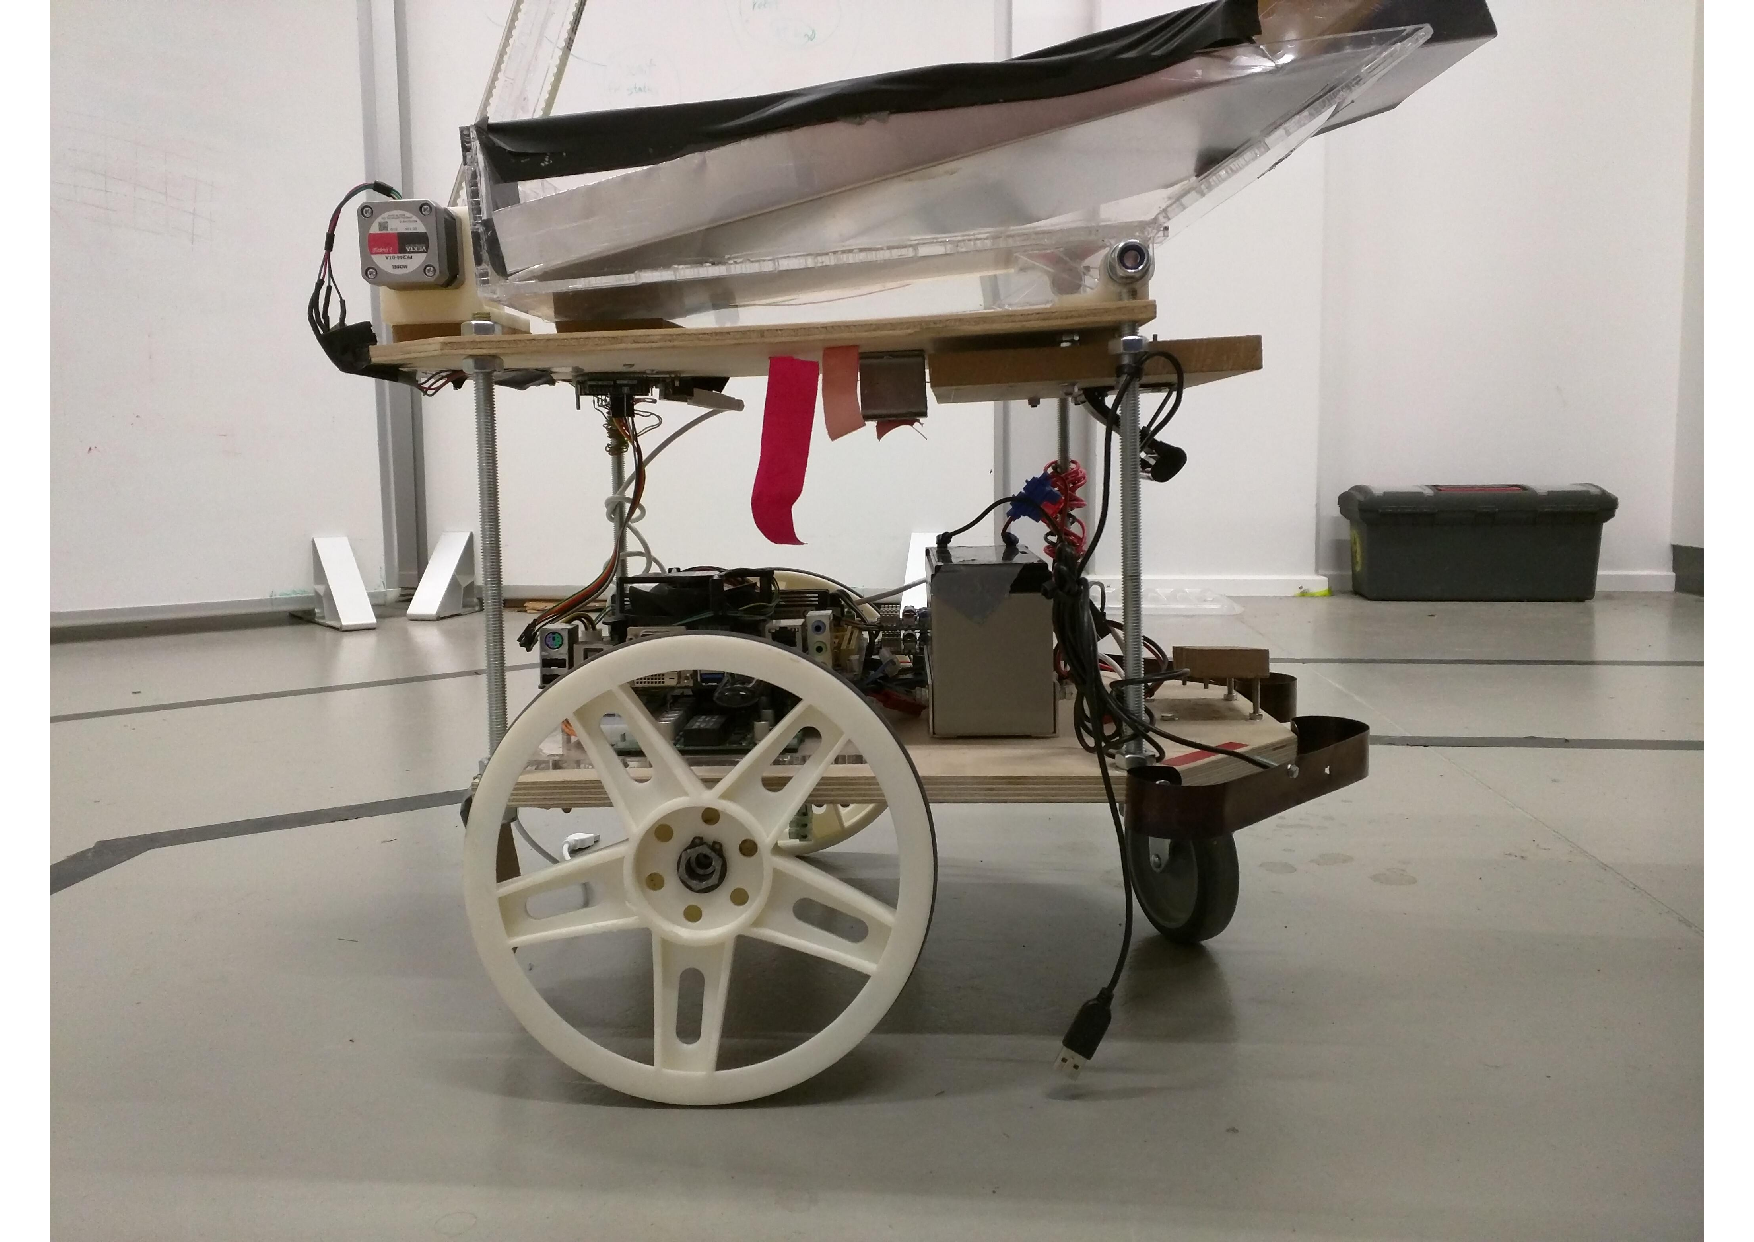
\includegraphics[width=0.7\textwidth]{frobit_profile}
	\caption{FrobitPro Robot}
	\label{fig:frobit}
	\end{figure}
\textbf{The main components for the tipper:}
\begin{itemize}
	\item PK-244-01A Bipolar Stepper motor
	\item Arduino UNO
	\item L298N dual H-bridge control board (Self-obtained)
	\item 2x Microswitch w/arm as end-point sensors for the motion
\end{itemize}   

To obtain valuable information about the surrounding environment, following 
sensors were used:
\begin{itemize}
	\item Sick LIDAR laser scanner
	\item VectorNav	 IMU
	\item Logitech Webcam
\end{itemize} 

The use of these sensors will be described in the appropriate sections. The IMU 
and LIDAR was on lend from the student library.\\
\\
\textbf{Modifications}\\
Along the development and testing phase of the project it was discovered that 
custom hardware modifications was necessary for the sensors to be mounted 
properly to the robot, in regards to protection of the sensors and be able to 
make proper use of these.\\

It was decided pre-hand that it was not allowed to make adjustments(e.g. 
cutting and drilling) in the base plate of the robot, of which it was chosen 
that the line-following camera would be mounted below the tipper without 
obstructing the LIDAR's field of view. This can be seen in figure 
\ref{fig:webcam_mr}.
\begin{figure}[H]
	\centering
	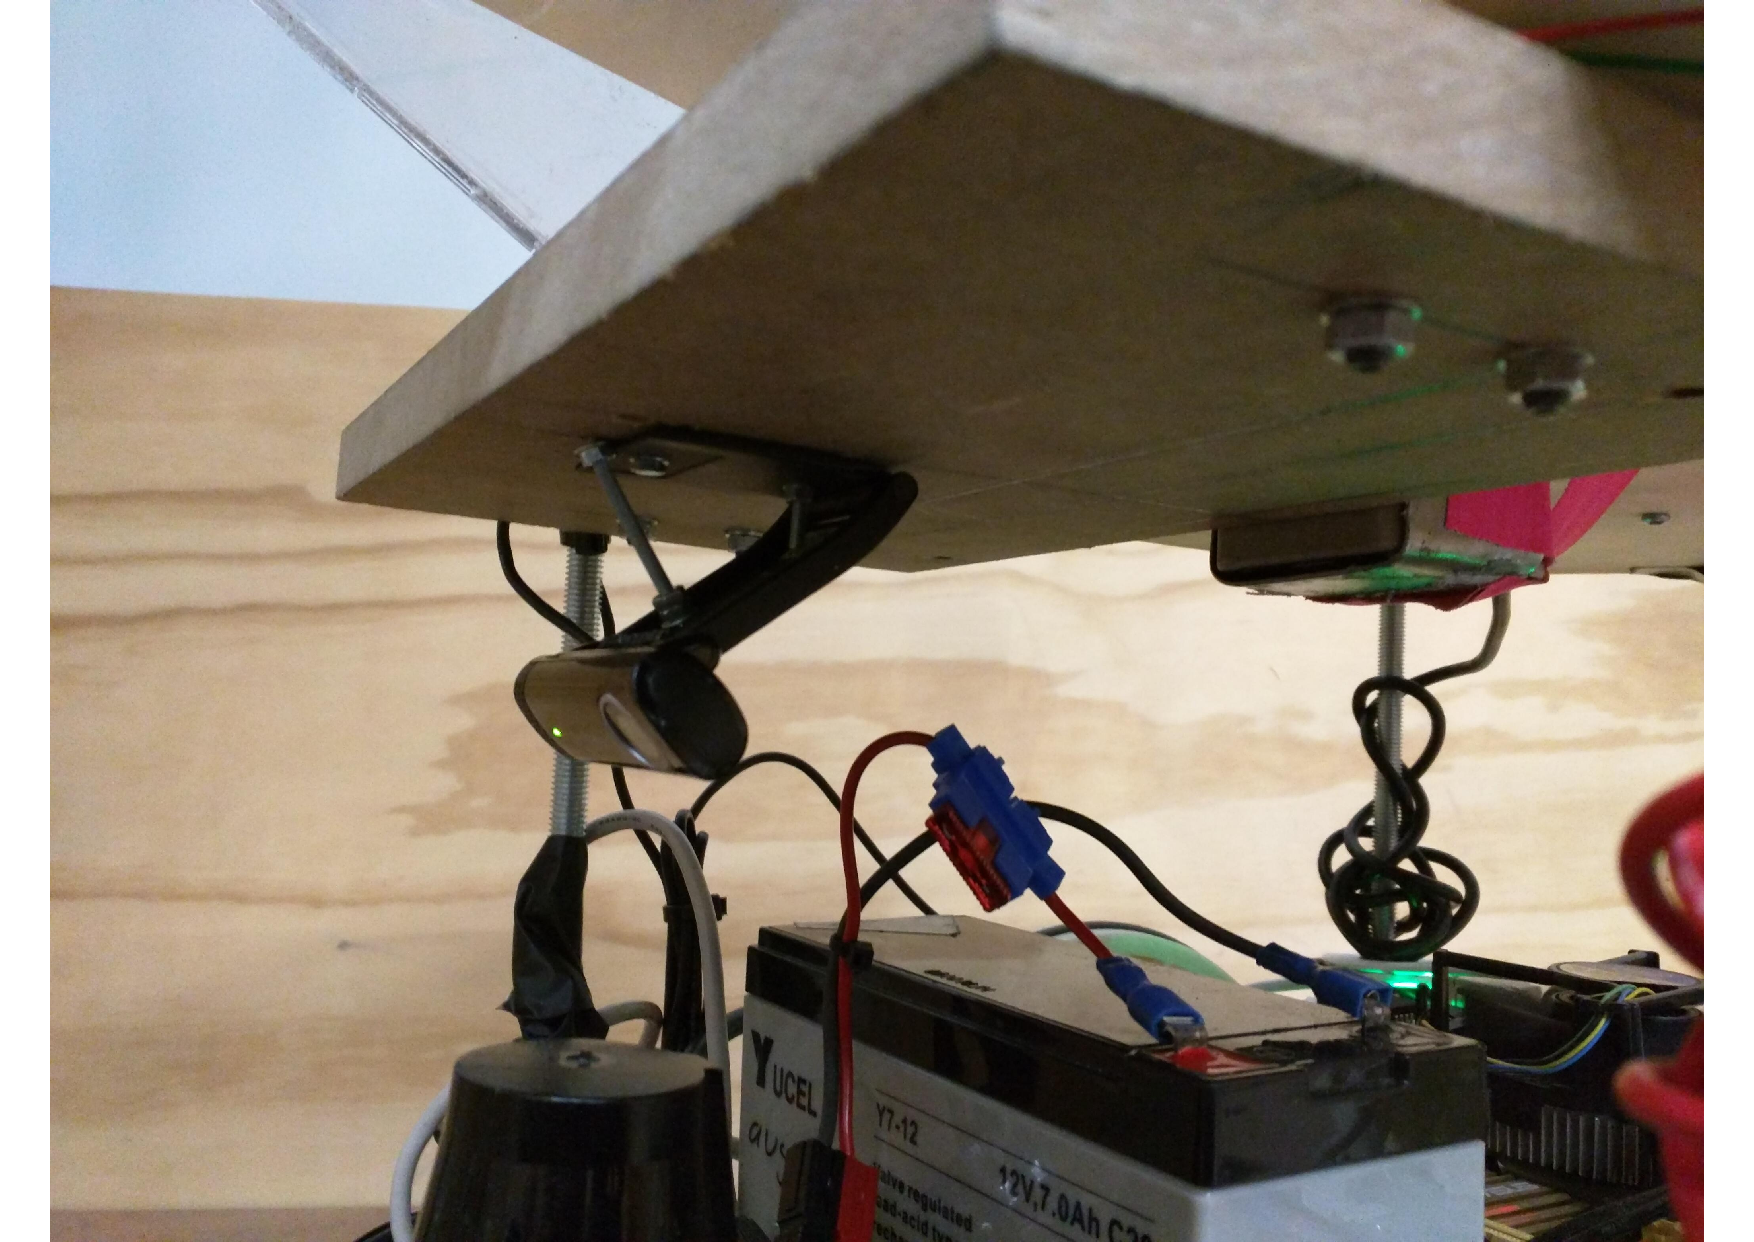
\includegraphics[width=0.7\textwidth]{webcam_mr}
	\caption{Line-following/QR detection camera}
	\label{fig:webcam_mr}
	\end{figure}
The previous use of an IMU on the robot had a remaining mount. With duct tape 
this was firmly attached. This can also be seen in figure \ref{fig:webcam_mr} 
in the background.
\begin{figure}[H]
	\centering
	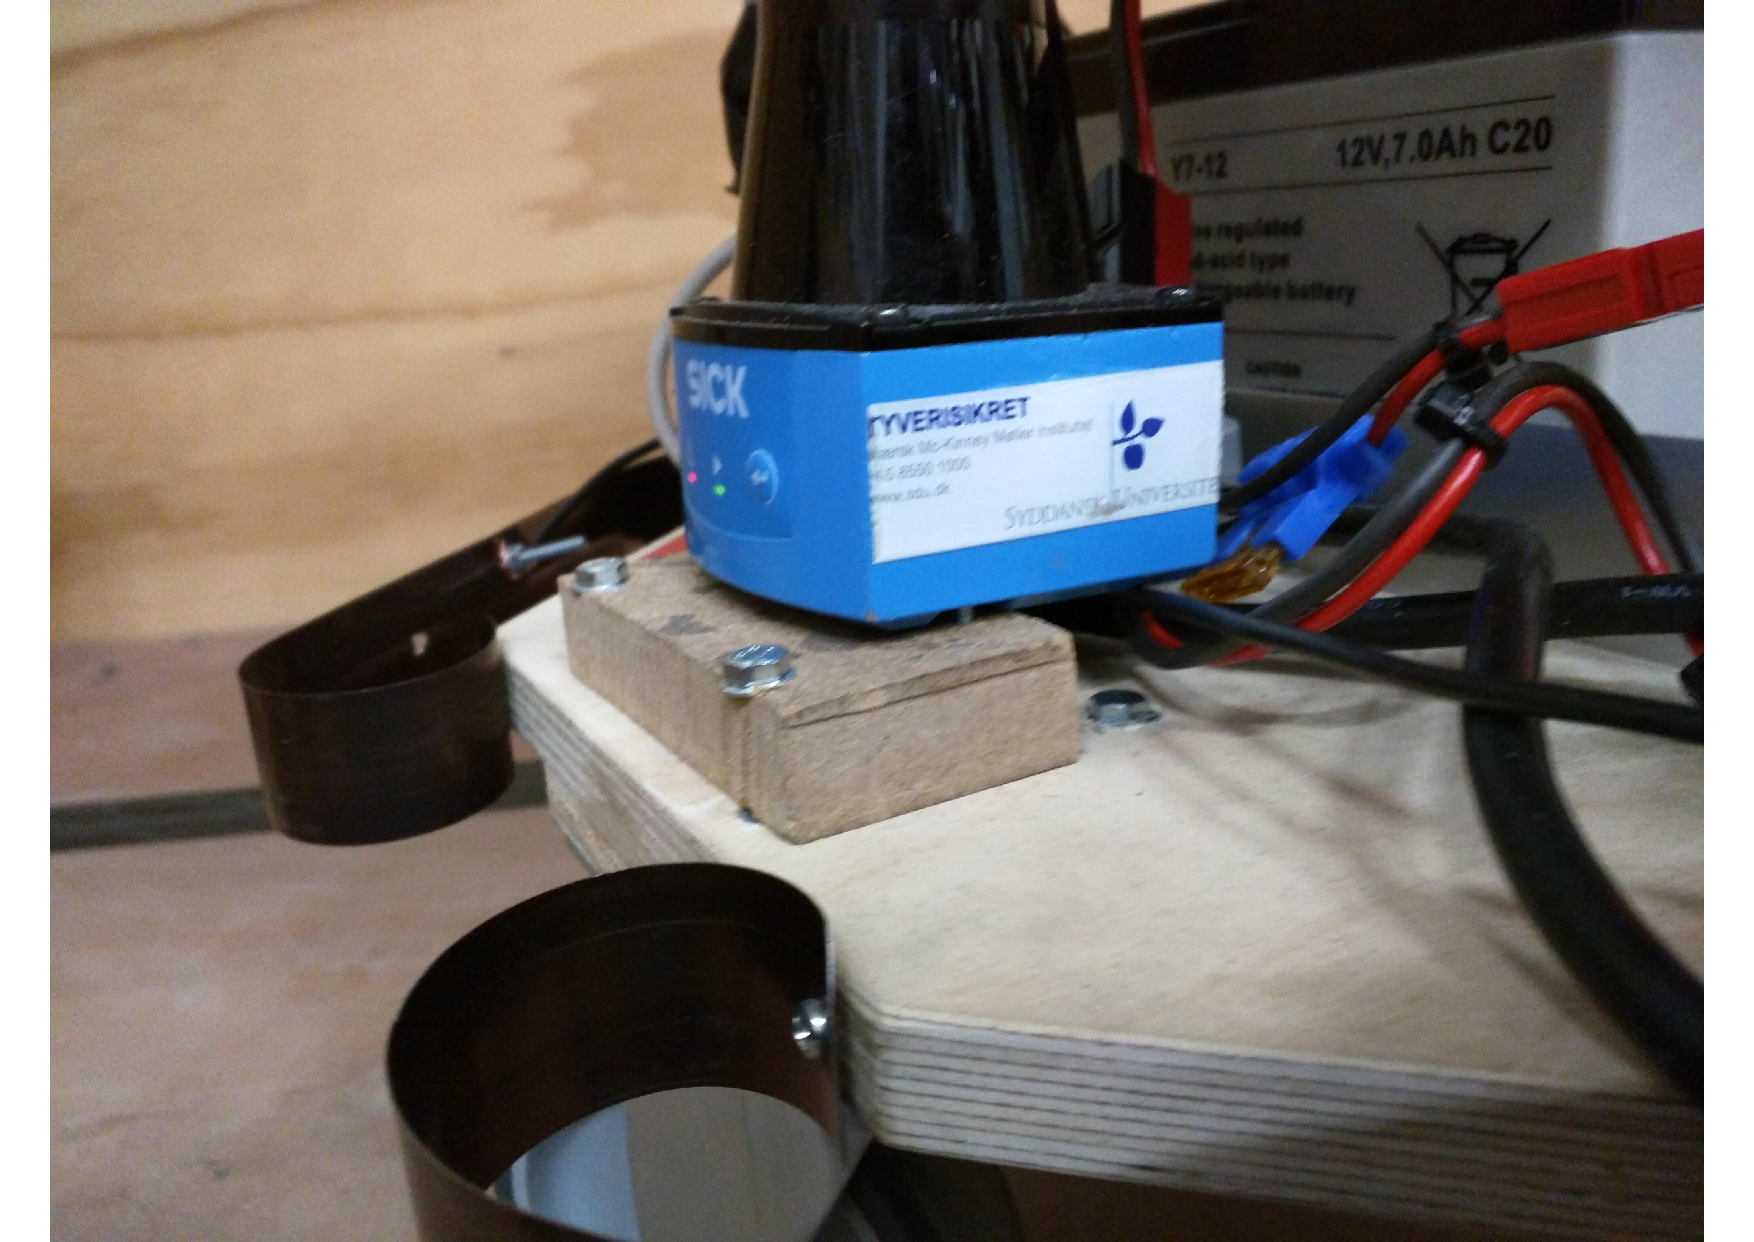
\includegraphics[width=0.7\textwidth]{lidar}
	\caption{Lidar laser scanner}
	\label{fig:lidar}
\end{figure}

In the preliminary tests, the Lidar was put on a wooden board in front of the 
robot to get as much use of the 270 degrees sensor as possible. 
Experimentally and in regards to the price of this sensor, it was later chosen 
to move it within the robot base to avoid any mishaps during an unforseen 
collision. See figure \ref{fig:lidar}. This obviously sacrifices some of the 
sensor angle.


The Arduino and H-bridge for the tipper control was mounted close to the 
stepper motor as shown in figure \ref{fig:arduino}. After some 
testing/collisions with the other robots, the usb plug of the arduino board had 
to be reattached and the board was therefore moved so nothing would interfere 
with the usb plug during runs. 

\begin{figure}[H]
	\centering
	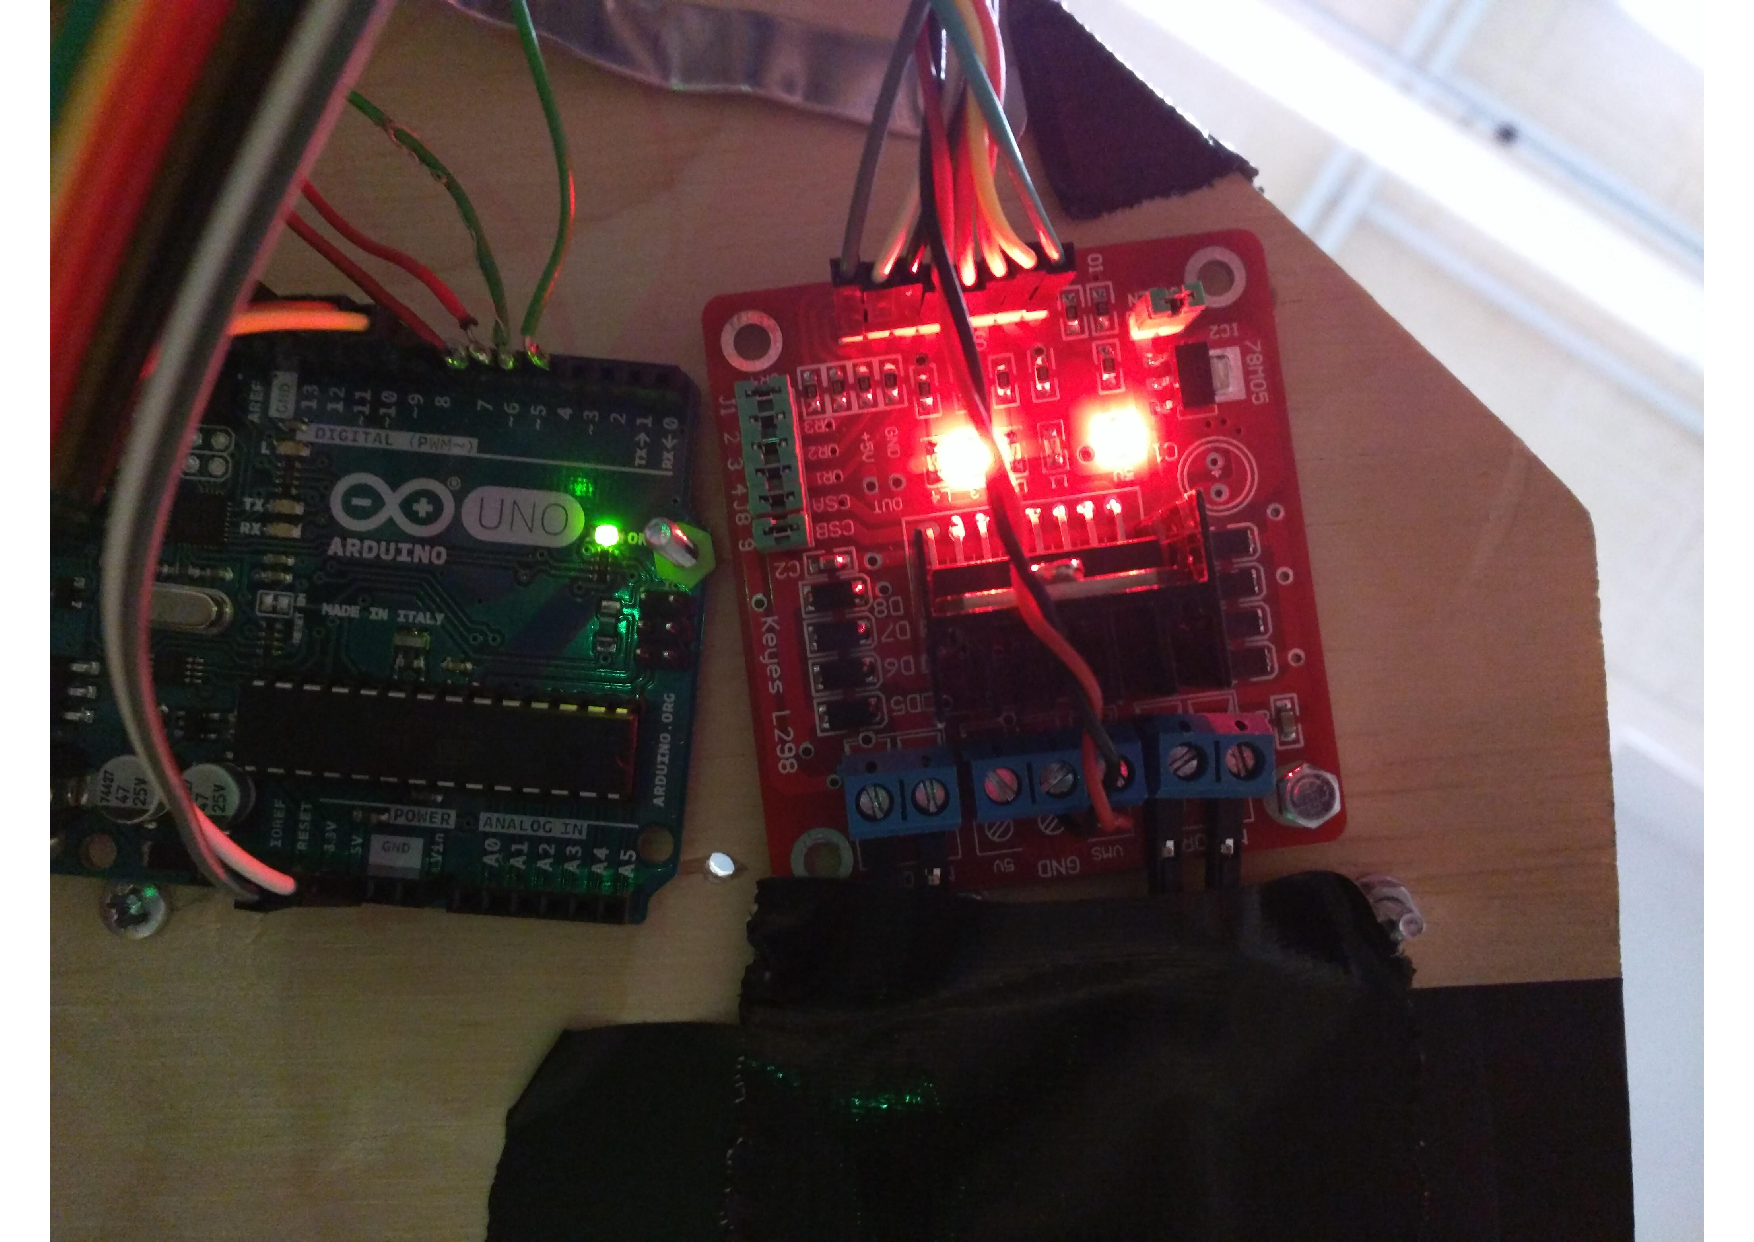
\includegraphics[width=0.7\textwidth]{arduinoandhbridge}
	\caption{Arduino and H-bridge mounted on the robot}
	\label{fig:arduino}
\end{figure}

During docking sessions in the dispenser/charging station, it was discovered 
that attaching a bumper-like system would increase the angle of which the robot 
could enter the charging station thus reducing the strictness of localization 
for going to the charger. The bumper idea can be seen in 
\ref{fig:bumper}.  


\begin{figure}[H]
	\centering
	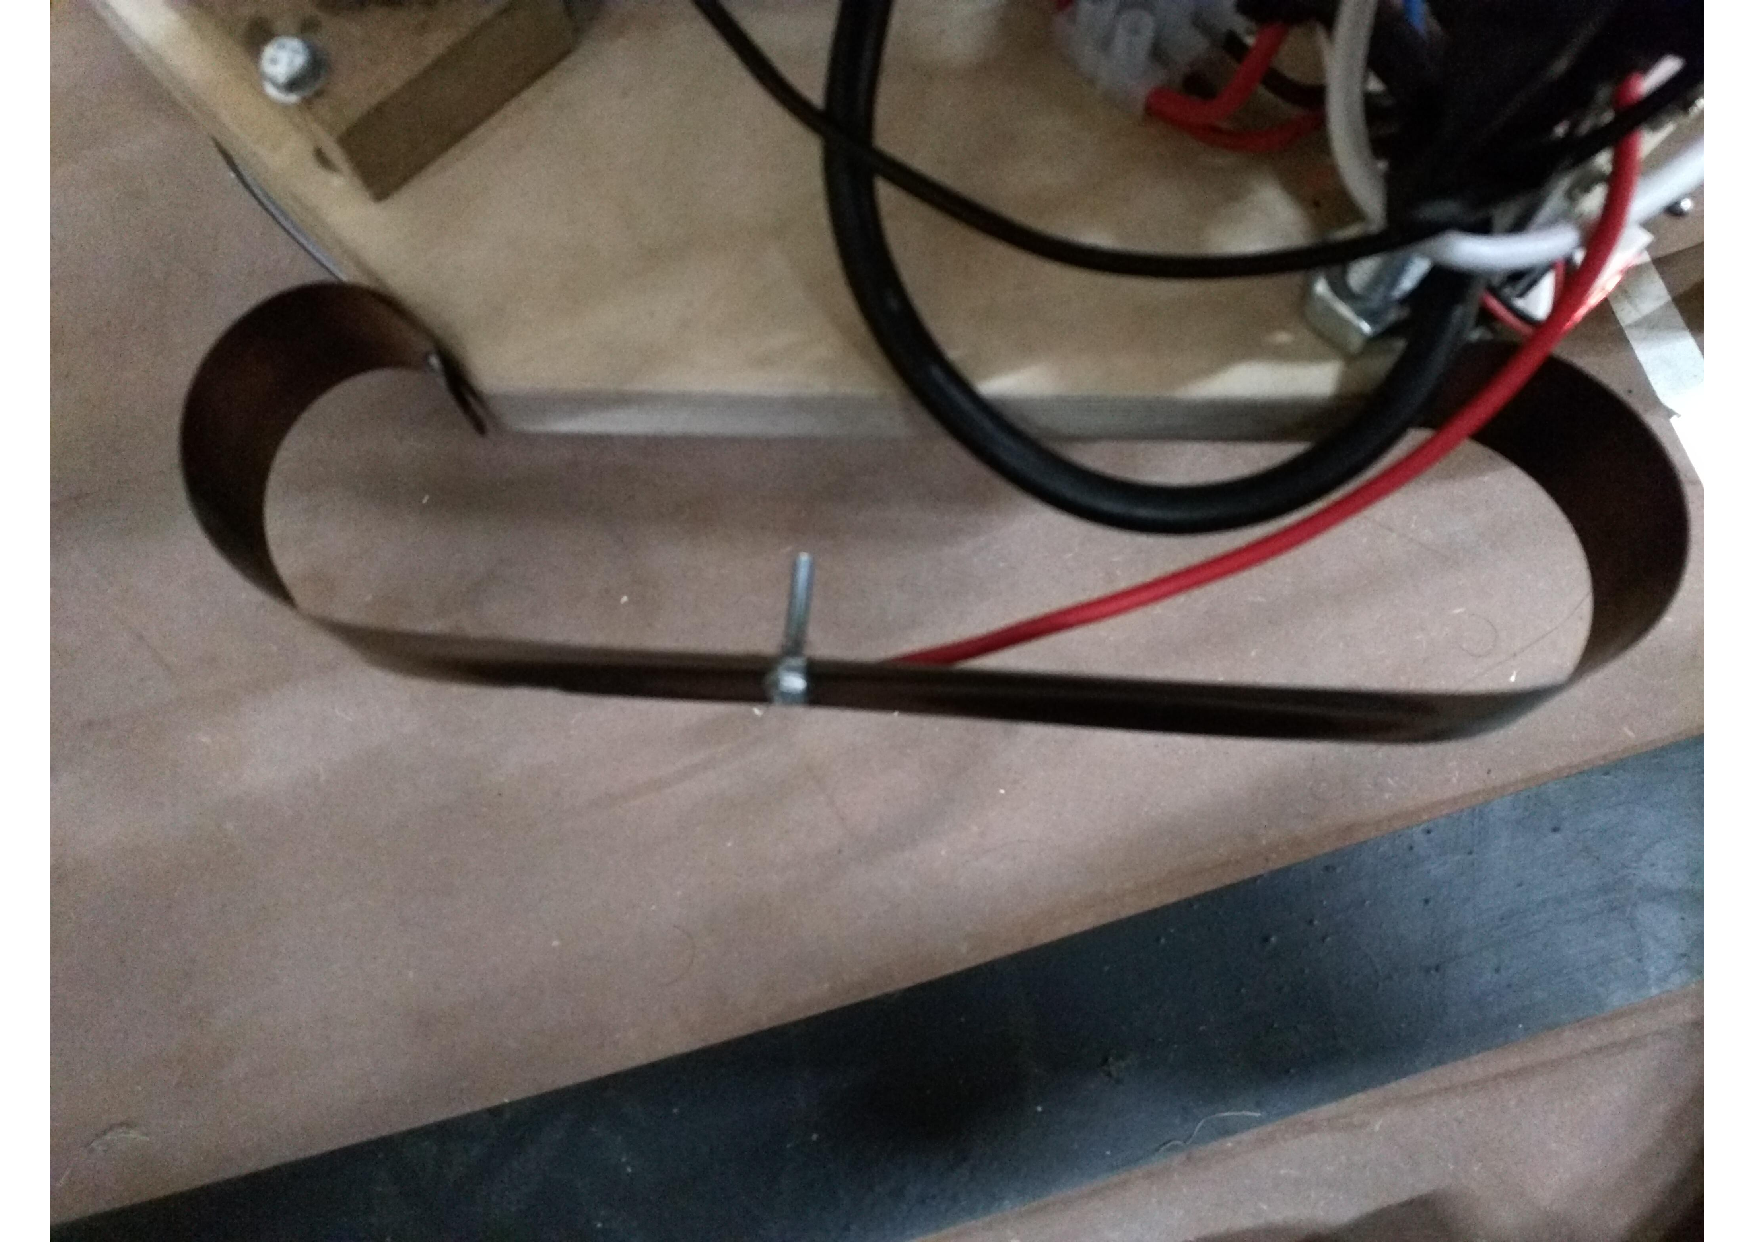
\includegraphics[width=0.7\textwidth]{bumper_mr}
	\caption{Bumper on the Mobile robot}
	\label{fig:bumper}
\end{figure}
Finally the plexiglas tray on top of the robot was found inadequate to deliver 
all bricks at the conveyor belt, so an aluminium insert was created. To ensure 
that the bricks were delivered to the conveyor belt and not next to it, this 
insert was created with a narrow tip, as seen in \ref{fig:tray}

\begin{figure}[H]
	\centering
	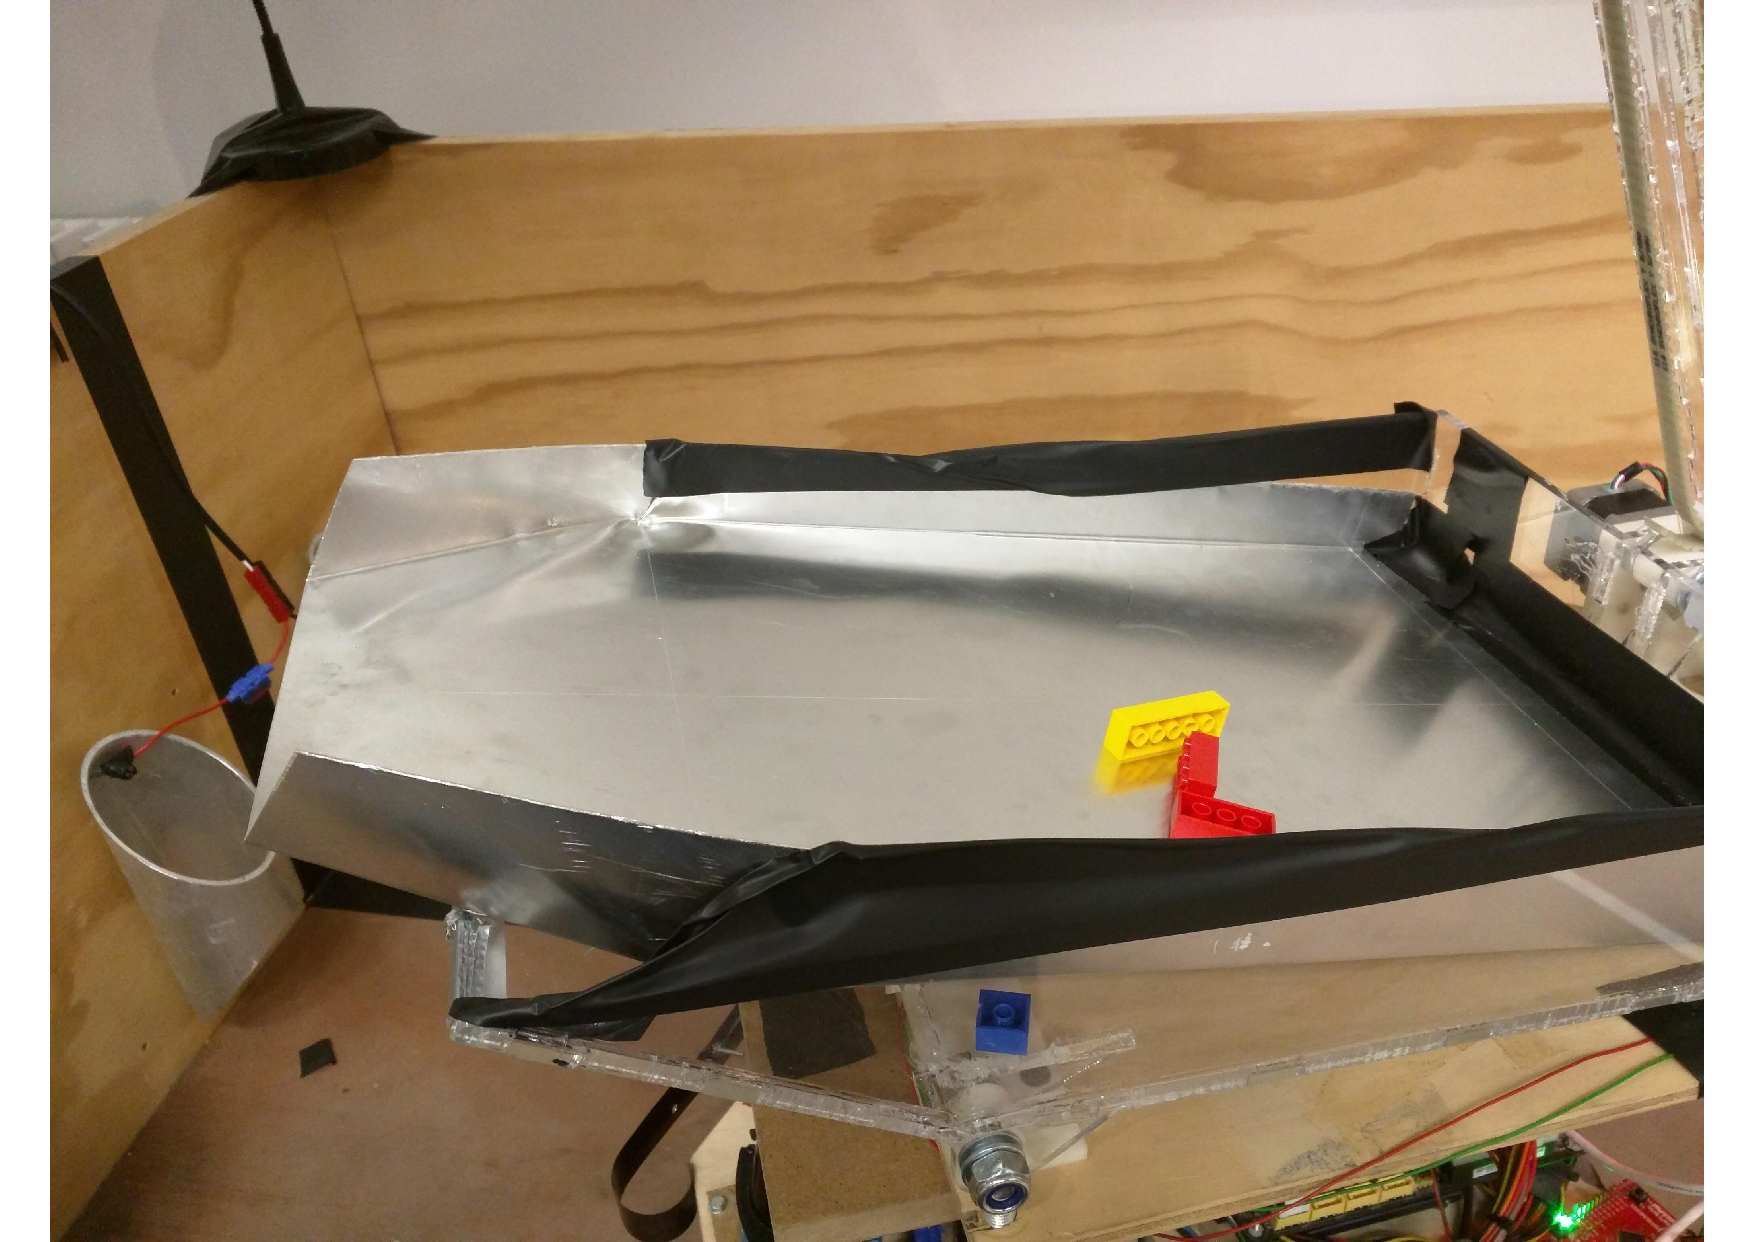
\includegraphics[width=0.7\textwidth]{trayside}
	\caption{Aluminium tray insert on the mobile robot}
	\label{fig:tray}
\end{figure}

% section hardware (end)
%!TEX root = ../../../main.tex
\section{Frobomind} % (fold)
\label{sec:mr_frobomind}

\textbf{Someone}

A shord tesciptiotion of FroboMind, what it is, the benefit of using it in comparison to a purely ROS based system, and how we use it now...

	\subsection{Frobomind interface} % (fold)
	\label{sub:mr_frobomind_interface}
	The frobomind interface is in charge of transform the hardware sensors values into ROS messages that can be used by the user.
	This is implemented as a ROS package given inside of the frobomind framework.
	A small modification in this package has been made so the status of the battery can be read.
	This allows the robot to create subrutines of charging when needed and continuing with the previous task when charged.
	% subsection frobomind_interface (end)
% section frobomind (end)


%!TEX root = ../../../main.tex
\section{Flow control overview} % (fold)
\label{sec:mr_flow_control_overview}
As explained in the chapter \ref{chap:mes_server_chapter}, the MES server sends an order and the clients have to read it and act consequently.
In the case of the mobile robot, there is a node in charge of do all the necessary steps in order to complete the order.

The flow control of the mobile robot is depicted in the figure \ref{fig:flow_control}.
This is:
\begin{enumerate}
	\item Wait for an order from the MES server.
	\item Read the order and go the brick dispenser to get some bricks.
	\item Go the the conveyor stated in the order.
	\item Tell to the MES server to activate the conveyor and unload the bricks previously picked up.
	\item Go to the position in which the robot of the workcell leave the order.
	\item Wait for the robotic arm to finish the order.
	\item Go to charge.
\end{enumerate}

\begin{figure}[htb]
	\centering
	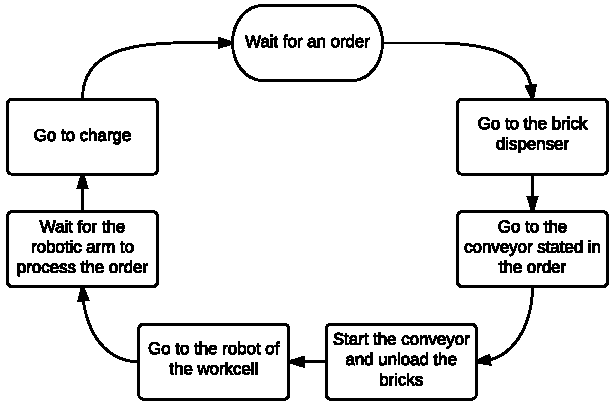
\includegraphics[width=0.75\textwidth]{flow_control}
	\caption{Flow control of the main node in the mobile robot}
	\label{fig:flow_control}
\end{figure}

This process is handled by the \emph{main node}, and this is the highest abstraction level in the control of the robot.
It is responsible of coordinate and actuate a second layer of abstraction which, at the same time, will be responsible of directly actuate the hardware.
The communications between the \emph{main node} an the second layer of abstraction, is shown in the figure \ref{fig:main_connections}.

\begin{figure}[htb]
	\centering
	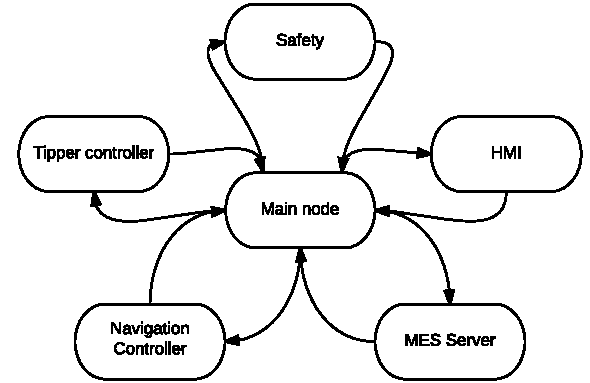
\includegraphics[width=.75\textwidth]{main_connections}
	\caption{Connections of the main node}
	\label{fig:main_connections}
\end{figure}

The main node has also an internal state of the robot represented in three states: \emph{idle}, \emph{auto} and \emph{manual}. 
The mode \emph{idle} means that the robot is not moving or executing any action. 
The mode \emph{auto} means that is processing an order and, consequently, it can be moving. \emph{Manual} stands for when the robot is being moved manually with the HMI. 
The states are intrinsically exclusive and the robot can only be controller manually if the robot is not processing an order.
This avoids the possibility of the user to interfere in the order status increasing the stability and reliability.

The connections are bidirectional and their functions are:
\begin{enumerate}
	\item \textbf{Safety}: Reads the state of the different sensors in the robot that measure the possibility of harm the robot and, if in danger, sends a signal to stops all the actuators.  
	\item \textbf{HMI}: This can change the state of the robot to \emph{auto} to start/continue an order, to \emph{idle} to pause the current order or to \emph{manual} if the user wants to control the robot manually. On the other hand, the main node can tell the HMI (1) its position and (2) the actions being carried out in that moment. This is that in the HMI is shown if the robot is, for example, inside the box and following the line or doing a relative movement.
	\item \textbf{MES server}: The main node reads the order sent and starts the new hierarchy of actions. Also the main node can send messages to the MES in order to activate other agents controlled by this.
	\item \textbf{Navigation controller}: As will be explained in the sections \ref{sec:mr_navigation_controller}, it is responsible of, knowing the current position of the robot, calculate a path to the desired position and perform it. The main node can receive from it when the robot has reached the desired position.
	\item \textbf{Tipper controller}: Handles the position of the tipper assembled in the robot. The controller can talk to the main node to tell when has finished the desired movement.
\end{enumerate}

% section flow_control_overview (end)


%!TEX root = ../../../main.tex
\section{Sensors and data processing} % (fold)
\label{sec:mr_sensors_and_data_processing}

	\subsection{Camera processing} % (fold)
	\label{sub:mr_camera_processing}
	

	\begin{figure}
        \centering
        \begin{subfigure}[ht!]{0.296\textwidth}
            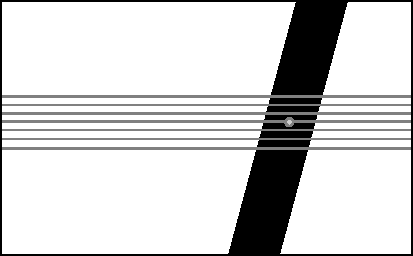
\includegraphics[width=\textwidth]{figs/mr_camera_processing_1}
            \caption{Clear detection of the line}
            \label{fig:mr_camera_processing_1}
        \end{subfigure}
        \hspace{40pt}
        \begin{subfigure}[ht!]{0.296\textwidth}
            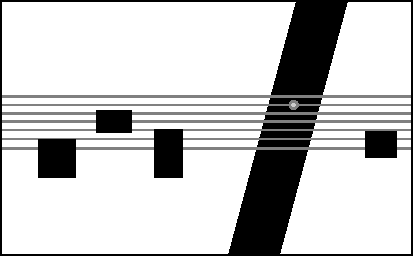
\includegraphics[width=\textwidth]{figs/mr_camera_processing_2}
            \caption{Detection when noise in the image}
            \label{fig:mr_camera_processing_2}
    	\end{subfigure}
    	\begin{subfigure}[ht!]{0.296\textwidth}
            
\includegraphics[width=\textwidth]{figs/mr_camera_processing_3}
            \caption{Detection when crossing line}
            \label{fig:mr_camera_processing_3}
    	\end{subfigure}
    \caption{Representation of possible cases when detecting the line}
    \end{figure}

	% subsection camera_processing (end)

	\subsection{Lidar processing} % (fold)
	\label{sub:mr_lidar_processing}
	
	% subsection lidar_processing (end)

	\subsection{Combined frobit odometry} % (fold)
	\label{sub:mr_combined_frobit_odometry}
	Wheels + IMU
	
	% subsection combined_frobit_odometry (end)

% section sensors_and_data_processing (end)
%!TEX root = ../../../main.tex
%%---------------------------------------------------------------------------
\section{Mobile Robot Navigation \label{sec:navigation_sec}}
%%---------------------------------------------------------------------------

How the mobile robot navigates in general (system overview), and the discussion of its subsystems in details (why, how, how well):
\begin{itemize}
    \item Navigation Controller
    \item In-box navigation
    \item Out-of-box navigation
    \item Line following
    \item QR-code reading
    \item HMI
\end{itemize}
\subsection{In-box Navigation} \label{sec:in_box_navigation}
As per project description, the navigation inside the box is to be done based on SLAM. Due to complexity of the entire project and potential diversity of SLAM implementations, an open-source implementation of SLAM was chosen. More specifically the gmapping-package \cite{gmapping} which has a livid community of supporters and builds a ROS wrapper for “OpenSlam's Gmapping”\cite{openslam}. TF-Frames of Lidar, IMU and the robot base were set up, this allows for easy transformation between Lidar and odometry data, inside the package. Using these, the SLAM-Implementation uses a particle filter to sequentially build up a map of the area. By manually driving through the entire workspace, a map was created. 
\begin{figure}[H]
	\centering
	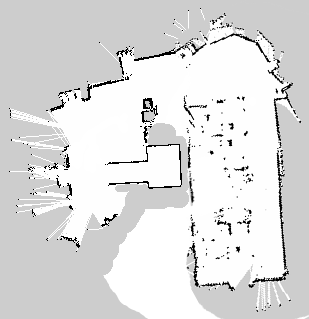
\includegraphics[width=0.5\textwidth]{slam_map}
	\caption{Slam Map}
	\label{fig:slam_map}
\end{figure}
Using the map-server package from the ROS 2D-Navigation Stack \cite{navigation_stack} the generated map was stored and is then broadcasted as a static map for localization. The AMCL (Adaptive Monte-Carlo Localization) package (which is also included in the navigation stack) then uses the static map, the lidar as well as odometry data to localize the robot while in free navigation. After tuning the parameters, AMCL worked fairly reliably for navigation both inside and outside the box.\\
\textbf{TODO: Describe move{\_}base}\\
Due to the box being fairly monotone in respect to the Lidar readings (clean, walls, no landmarks), precise navigation inside the box was sometimes not perfect. Also with multiple robots present in the box, issues, especially when trying to charge occurred. To ensure reliability of charging, a backup behaviour was added, when the charging failed using move{\_}base. For this a line was added, using the already implemented Line Following behaviour. The move{\_}base is used to navigate the robot to the start of the charging line. Then the robot follows the line until a pre-specified distance from the wall using Lidar. Having a main and a backup behaviour proved to be sufficient for reliable charging\\
\textbf{TODO: IS THAT REALLY SO?}
%!TEX root = ../../../main.tex
\section{Navigation Controller} % (fold)
\label{sec:mr_navigation_controller}
Using the processed information from the sensors and the different kind of navigations, the robot is able to move and satisfy all the requirements from the project.
In this section the \emph{navigation controller} is explained.
This is in charge of finding the path, and actions associated to said path, given two nodes.

\subsection{Navigation state representation} % (fold)
    \label{sub:mr_navigation_state_representation}
    In order to navigate from one position to the desired one, a graph of the possible states in which the robot is stopped or idle has been represented.
    This graph depicts all the possible states of the mobile robot in which the robot has not movement along with their associated transference functions. 
    These are other states in which the robot is moving or changing its state and that in this project will be referred as \emph{skills} (Section \ref{sub:skills}).
    In the figure \ref{fig:mr_graph} the graph of the project is shown.
    
    \begin{figure}[H]
        \centering
        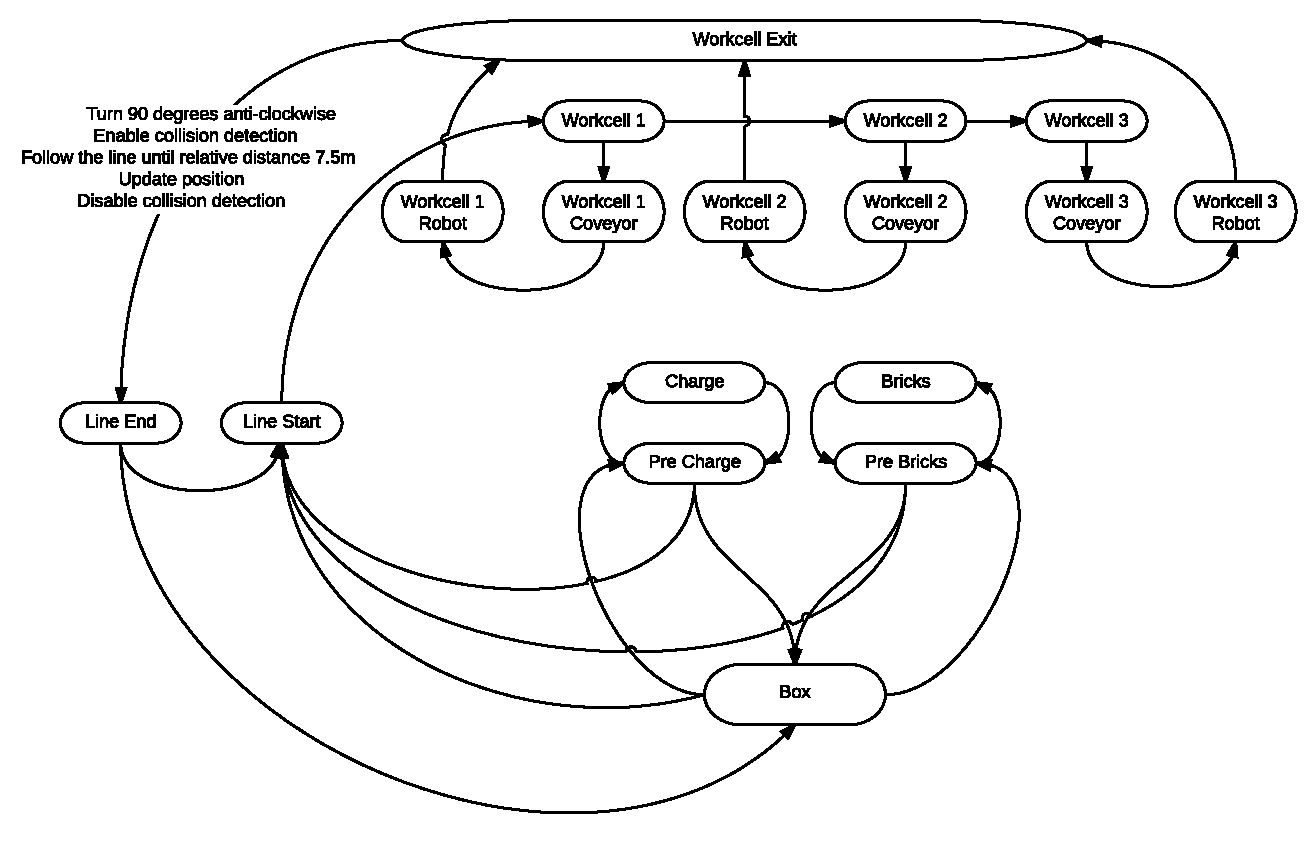
\includegraphics[width=\textwidth]{figs/mr_graph.pdf}
        \caption{Graph representation adopted in the project}
        \label{fig:mr_graph}
    \end{figure}

    As an example, in the transference between the node \emph{"Workcell Exit"} and \emph{"Line End"}, the associated conditions are shown. 
    These are: first, needs to \emph{turn 90 degrees clockwise}, then \emph{follow the line until the QR "line\_end"} is detected, all this done with the collision detector turned on and changing the internal position of the robot in the end.
    % subsection navigation_state_representation (end)

    \subsection{Skills} % (fold)
    \label{sub:skills}
    As stated before, the skills are available actions to transfer the robot from one navigation state to another. They let the robot change its state and position.
    The implementation is based on a couple between one of the navigation types and some information from the sensors used as a condition.
    The skills designed and implemented are:
    \begin{itemize}
        \item Follow the line until desired QR
        \item Follow the line until desired LIDAR distance
        \item Follow the line until desired relative distance
        \item Linear relative move
        \item Angular relative move
        \item Go to free position
        \item Detect obstacles
        \item Wait
        \item Specialized charging skill
        \item Initialising the AMCL 
    \end{itemize}    
	An example of the skills associated with the transition from one node to another is shown in figure \ref{fig:mr_graph}. The skill list shown only facilitate the transfer when exiting from work-cell 1, due to the use of the follow line until relative distance. This distance will be different for each work-cell.

The navigation skills have previously been described. The specialized charging skill combines multiple of the other skills. Initially the robot moves to a position in free space. Then it follows a line until a certain LIDAR distance. Here it waits 10 seconds to see if the battery level has risen. If it has risen the state is set to charge. Otherwise the robot reverses and restarts the process. \\
The last skill, initialising the AMCL, is used when the robot transitions from the line navigation to free navigation. This is necessary because the AMCL looses its position when the robot moved into the robot cells.
	
	
    % subsection skills (end)

    \subsection{Graph search} % (fold)
    \label{sub:mr_graph_search}
    In order to find the most optimal path between two nodes in the graph a graph search algorithm has been implemented.
    All the transfers between states have an associated cost which is used by a Breadth First Search (BFS).

    The BFS is an algorithm of searching in graphs that explores all the neighbours of the root, then the neighbours of this ones etc.
    BFS is a complete search algorithm and optimal meaning that will always find the optimal solution.
    In this case as the cost between nodes is a given distance, the BFS will always find the shortest path.
    
    The negative part of the BFS is the space complexity but due to the graph being rather small, the search time is in the order of milliseconds.
    % subsection artificial_intelligence (end)
% section navigation_controller (end)

%!TEX root = ../../../main.tex
\section{Tip controller} % (fold)
\label{sec:mr_tip_controller}

The purpose of tip controller is to create a simple and effective way of 
delivering a large amount of LEGO bricks to the conveyor belt autonomously. 
This is done by controlling the mounted belt drive with a stepper motor, an 
H-bridge and a Arduino microcontroller. To control the limits of tipping 
mechanism, two microswitches were added(Tip down/tip up).\\

\subsection{Stepper controller} % (fold)
\label{sub:stepper_controller}
The PK-244-01A stepper motor is bipolar. This means that it requires (at least) 
four wires to control the two coils in contrast to a unipolar motor which has 1 
supply wire and usually only requires two control wires. 
The four wires are driven by the L298N dual 
H-bridge, powered by 12V from on-board pc power supply. Four control pins are 
connected to the 
Arduino and signals on these controls the motor wires. Consulting datasheet for 
the motor, a minimum of 4V, 1.2A is required to drive the motor. Timing is 
calculated as a minimum of 
3ms delay between steps in the timing diagram. To get an initial high torque 
from the motor, a half-stepping sequence was chosen and a ramp function was 
created to slowly start the motor and exponentially increase speed when the 
tip is in full motion. Due to friction in the system and less torque the 
full-step sequence was disregarded. The Arduino software has a built-in library 
for stepper motors, but this was found difficult to manage in regards to delay 
of the steps. 
% subsection stepper_controller (end)

\subsection{Arduino and serial communication} % (fold)
\label{sub:arduino_and_serial_communication}
Setting a general serial communication to the Arduino is straight-forward. The 
speed is chosen with regards to the ROS node and a serial connection is 
initialized with the \textbf{Serial.begin(speed)} command. The Arduino is set 
up to 
receive a character "u" for tipping(up), and "d" for leveling(down). When an 
action has successfully executed, a "d" (done) is returned to the ROS node.
% subsection arduino_and_serial_communication (end)


% section tip_controller (end)

%!TEX root = ../../../main.tex
\section{Safety system} % (fold)
\label{sec:mr_safety_system}
The safety in the mobile robot is intrinsic in all the nodes that allow its movement.
Additionally the Safety Eyes was supposed to be used to detect humans in the area close to the stairs. However due it not working, it was not being used.
There then are two aspects to talk about: (1) the \textbf{incident handler} based on the the given frobomind implementation. Based on certain inputs, an \emph{activation} signal is created, allowing the robot to move.
(2) On the other hand, the \textbf{obstacle detector} is used to feed another skill (see section \ref{sub:skills}) that changes the speed, or even stops, the robot depending on the distance of obstacles detected by the LIDAR.
This can be activated or disabled depending on the situation.
	\subsection{Incident handler} % (fold)
	\label{sub:mr_incident_handler}
	The incident handler is based in the \emph{simple incident handler} given inside of the frobomind framework.
	This system receives two signals: (1) the \emph{deadman} and (2) the \emph{critical fault}.
	When both signals are received correctly, the incident handler outputs another signal that \emph{enables the actuation}.
	This signal is directly received from the system that actually performs the actions that move the motors in the robot.
	Both signals are booleans with a time stamp and need two conditions to be approved:
	\begin{enumerate}
		\item As booleans, need to be true.
		\item As stamped, need to be received in an interval smaller than a threshold. In our system the signal need to be received in intervals inferior to 50 milliseconds.
	\end{enumerate}
	If both, \emph{deadman} and \emph{critical fault}, are received by the incident handler satisfying those conditions, the output signal \emph{actuation enable} will be published and the robot will move.
		\subsubsection{Deadman} % (fold)
		\label{ssub:mr_deadman}
		The deadman signal is used by the navigators to actually perform a movement.
		As stated previously, the signal needs to be sent in intervals lower to 50 milliseconds and be true.
		The deadman signal received in the incident handler doesn't contain information about who is the sender, but is not a problem due to the navigators are made so they are exclusive.
		This means, that only one deadman signal is received from one navigator.
		% subsubsection deadman (end)

		\subsubsection{Critical fault} % (fold)
		\label{ssub:mr_critical_fault}
		The critical fault signal is controlled by the main controller of the robot.
		This node, as explained in the section \ref{sec:mr_flow_control_overview}, controls among others the mode of the robot.
		Only in the modes \emph{manual} and \emph{auto} this signal is activated meaning that if the robot is in \emph{idle}, either because there was a critical fault in the robot or because manually was stopped, the robot cannot move.
		As stated previously, the signal needs to be sent in intervals lower to 50 milliseconds and be true.
		% subsubsection critical_fault (end)
	% subsection incident_handler (end)

	\subsection{Obstacle detector} % (fold)
	\label{sub:mr_obstacle_detector}
	Its function consist of reading all the distances information from the LIDAR and, given a detection angle and two thresholds (\emph{proximity alert} and \emph{colliding}), output a signal which will slow down or stop the robot.
	The obstacle detector is used inside of an skill (see section \ref{sub:skills}) so it can be activated or disabled when necessary.

	In practice the obstacle detector is only used in places where (1) there is a risk to crash and (2) its behavior doesn't affect to the main one.
	This means that, for example, inside of the robotic arm workcell it is disabled due to (1) the robot cannot crash with any moving agent and (2) due to the proximity to other static parts inside the workcell, it would be in the \emph{proximity alert} mode all the time. 

	% subsection obstacle_detector (end)

	The output of the obstacle detector can be three different exclusive states: (1) \emph{safe}, (2) \emph{proximity alert} and (3) \emph{colliding}. 
	The default mode is \emph{safe}, while the other two modes are enabled based on two thresholds.
	The thresholds are expressed in the same units as the distance received from the LIDAR being in our project 40 cm for \emph{proximity alert} and 15 cm for \emph{colliding}.
	When in \emph{proximity alert} the robot will slow down its movement (any) in a factor of 0.5 and when in \emph{colliding} will stop.

	The limitations of this system is that with the LIDAR being mounted in the front, only obstacles which are in the area of the LIDAR can be detected.
	So no obstacles in the sides and behind are detected and these movements are "blind".
% section safety_system (end)

%!TEX root = ../../../main.tex
\section{Human Machine Interface} % (fold)
\label{sec:mr_human_machine_interface}

Motivation for having one, capabilities, implementation, testing and results.

	\subsection{Web} % (fold)
	\label{sub:mr_web}

	% subsection web (end)

	\subsection{Physical devices} % (fold)
	\label{sub:mr_physical_devices}
	Talk here about the button too.

	% subsection physical_devices (end)

	\subsection{ROS Services} % (fold)
	\label{sub:mr_ros_services}

	% subsection ros_services (end)

% section human_machine_interface (end)

    %!TEX root = ../../main.tex
%----------------------------------------------------------------------------
\chapter{Robot Cell Design}\label{chap:robot_cell_chapter}
%----------------------------------------------------------------------------
Equipped with a robot manipulator, a gripper and a conveyor belt the task of the robot cell is to sort the Lego bricks delivered by the mobile robot. These are delivered to the conveyor belt which moves them closer to the camera and robot. Here the corresponding bricks ordered by the MES system should be picked and returned to the mobile robot. This is the task each robot cell has to fulfil, and just like in the case of the mobile platform, the process can be subdivided into smaller tasks, which we will introduce in the upcoming sections.


% Please keep sections separated in their designated folders and only reference them here using the input tag

%!TEX root = ../../../main.tex
%%---------------------------------------------------------------------------
\section{Hardware}
\label{sec:rc_hardware}
%%---------------------------------------------------------------------------
The following hardware elements was provided in each robot cell:

\begin{itemize}
	\item Kuka KR6 Robot
	\item PG70 Gripper
	\item Conveyor Belt with 3 phase 240V Motor
	\item ABB (ACS150-01E) Frequency Converter
	\item ABB (PM554) Programmable Logic Controller(PLC) for conveyor control
	\item SICK (M4000) Laser safety fence
	\item HD Webcam for Lego brick detection in 2D
	\item Kuka touch screen for HMI
\end{itemize}

The set-up for involved components will be discussed in details where appropriate. 

\subsection{Modifications}
The conveyor belt required some changes to be able to handle and control the flow of Lego bricks. First a funnel, see figure \ref{fig:funnel}, was added as a tip-off location for the mobile robot.

  	\begin{figure}[H]
        \centering
        \begin{subfigure}{0.48\textwidth}
			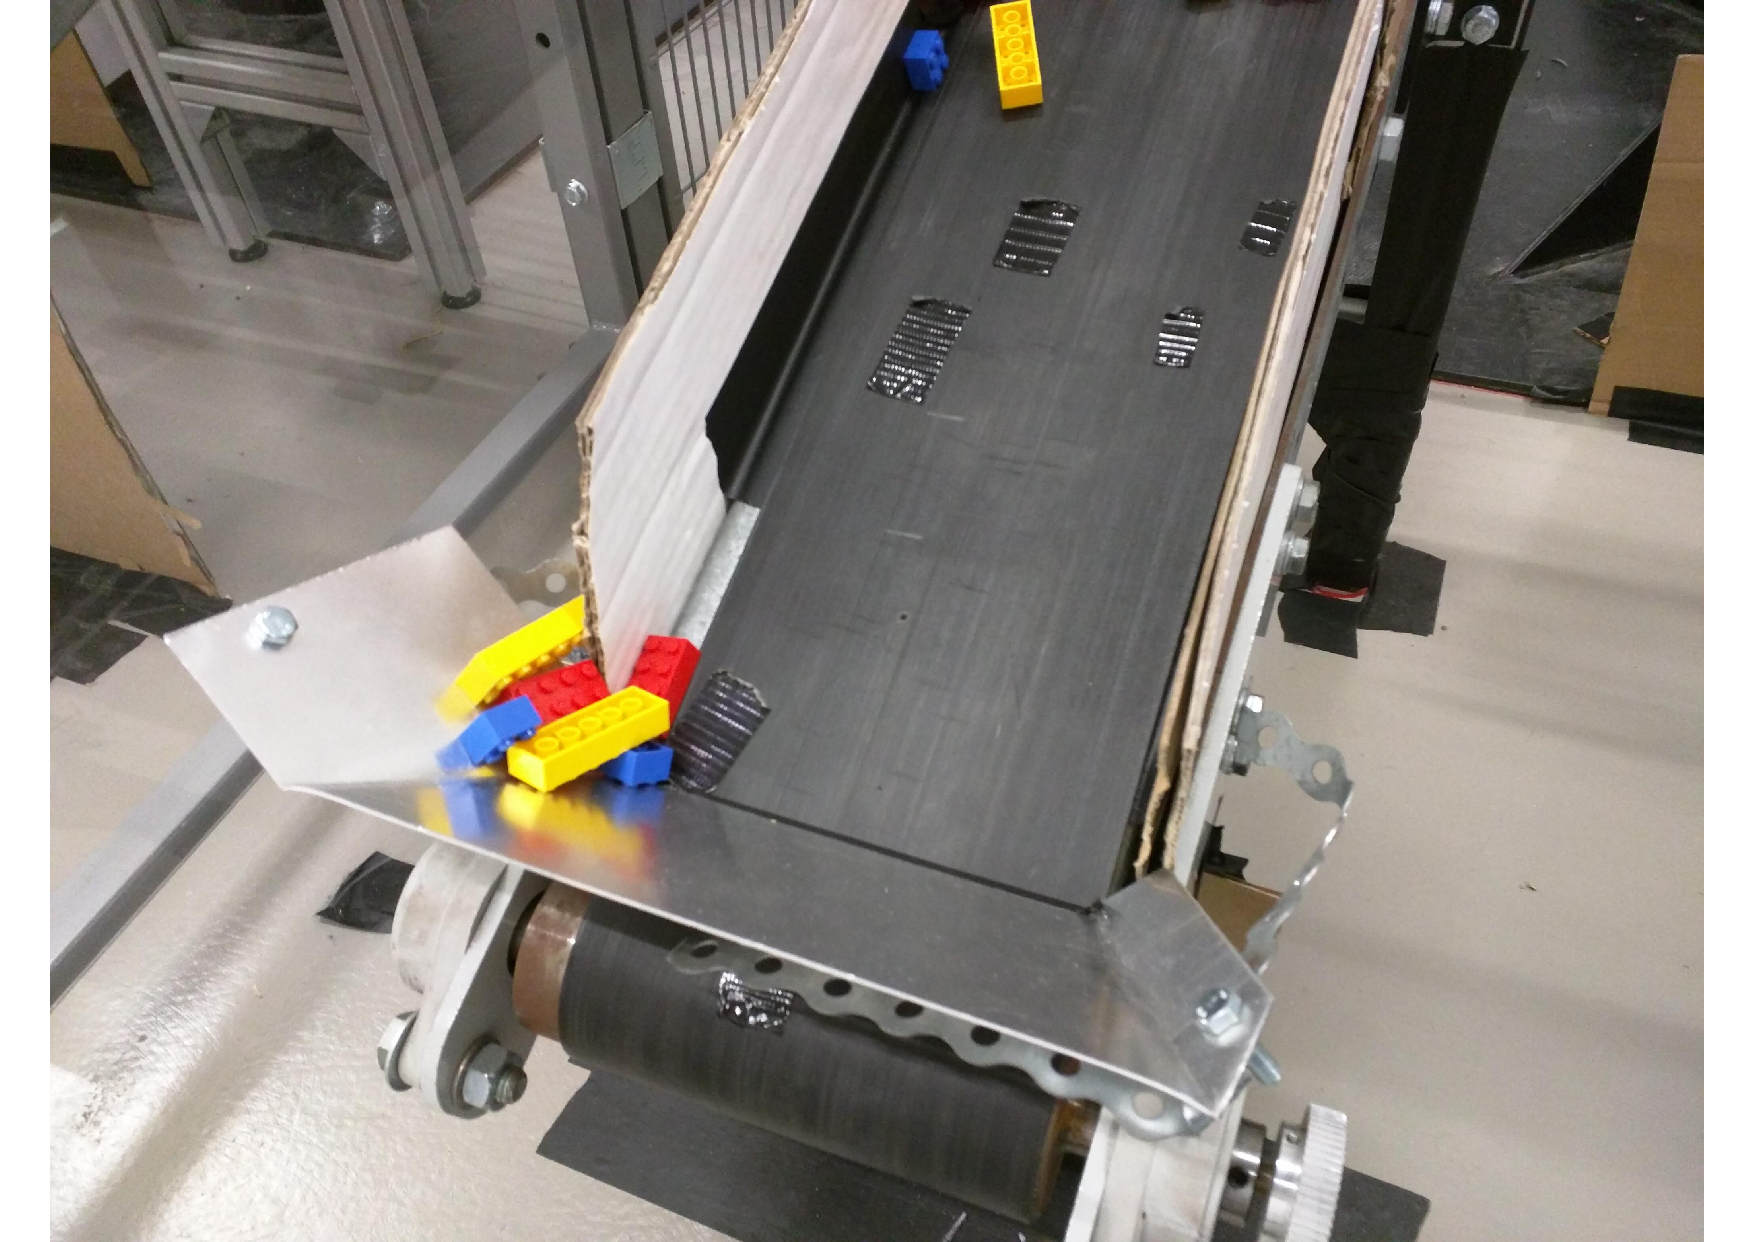
\includegraphics[width=1\textwidth]{funnel_rc}
			\caption{Funnel at delivery point for the mobile robot}
			\label{fig:funnel}
        \end{subfigure}
        \hspace{10pt}
        \begin{subfigure}{0.48\textwidth}
			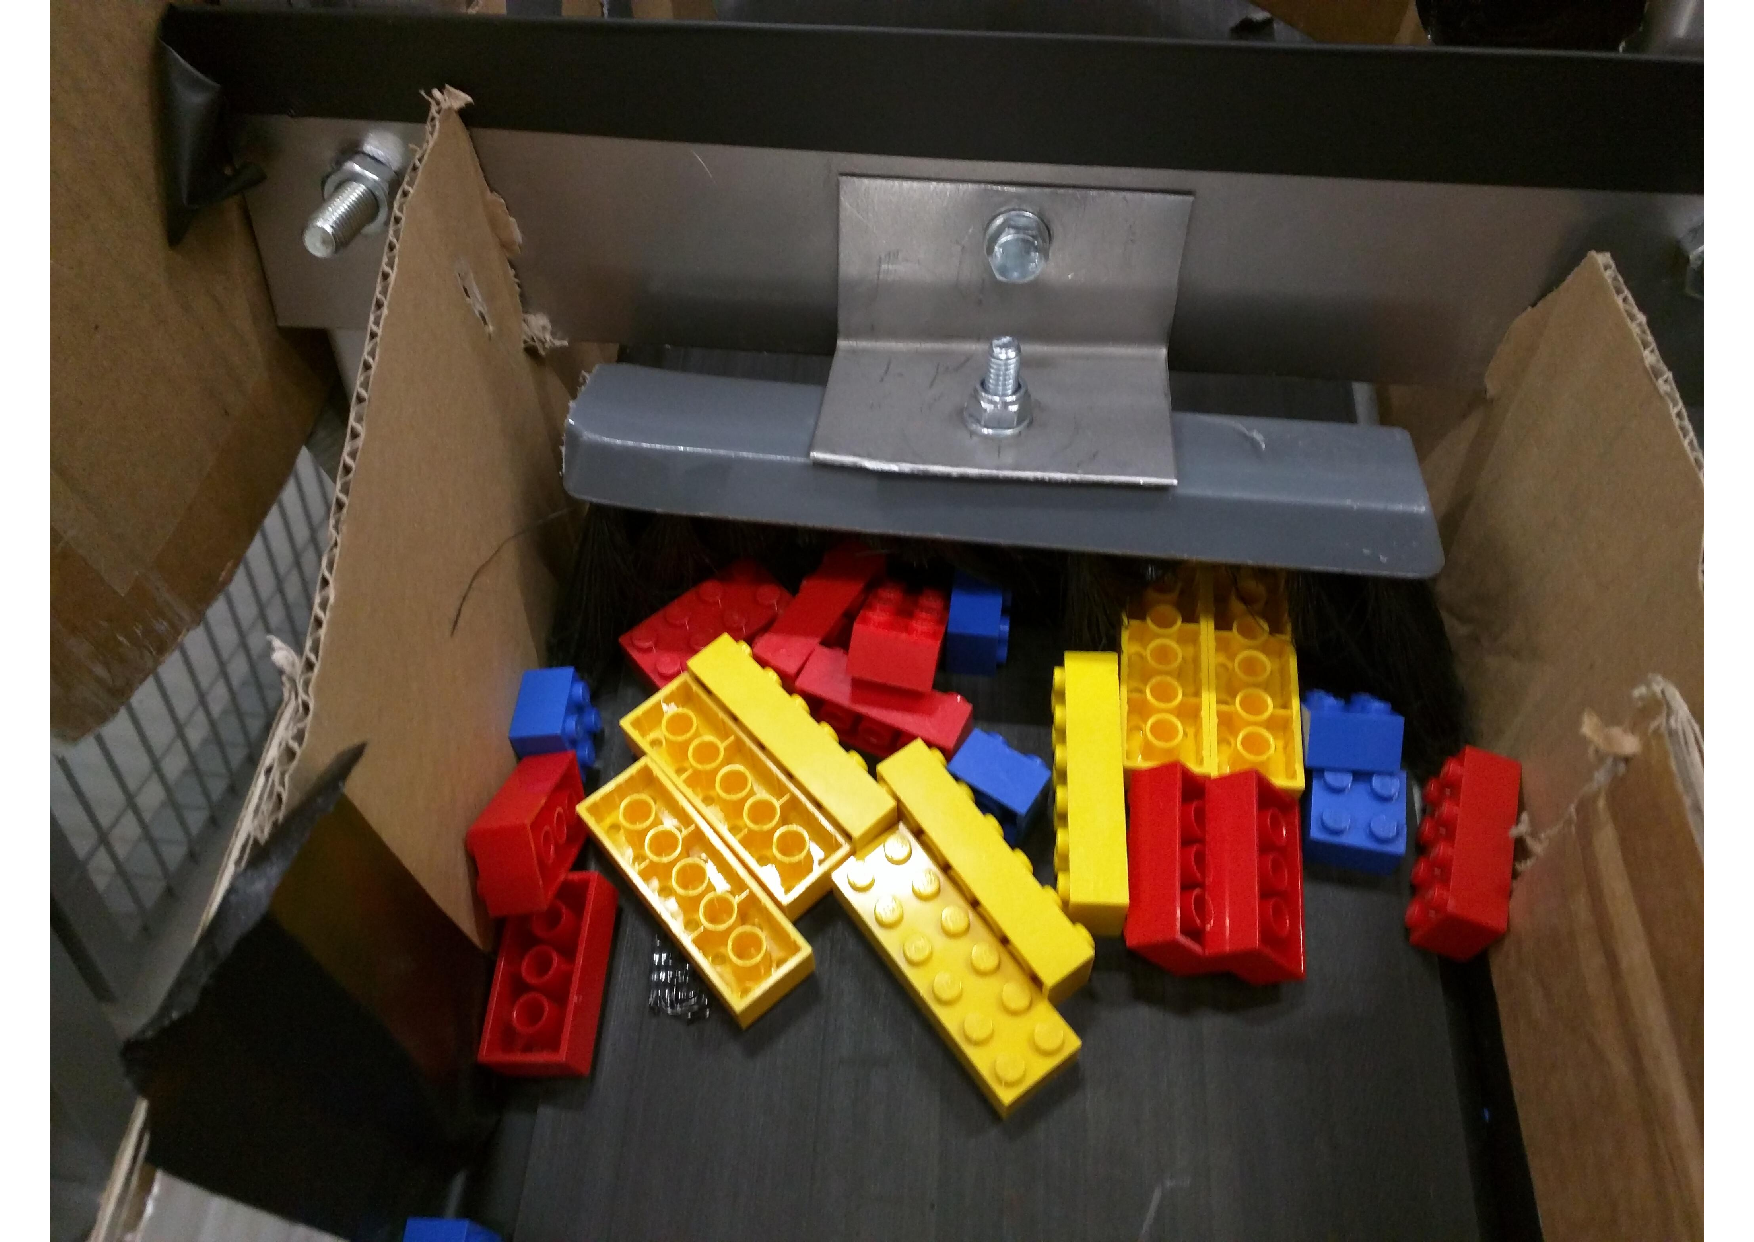
\includegraphics[width=1\textwidth]{brush_rc}
			\caption{Brush system to de-cluster the bricks}
			\label{fig:brush}
    \end{subfigure}
    \caption{Example of conveyor modifications}
    \end{figure}

Secondly, to avoid clustering and multiple layers of bricks a passive system consisting of a brush and cardboard was invented as shown in figure \ref{fig:brush}.

To provide the necessary friction to go through the system, duct tape was added at random places to the conveyor belt. See figure \ref{fig:duct_tape}.

  	\begin{figure}[H]
        \centering
        \begin{subfigure}{0.48\textwidth}
			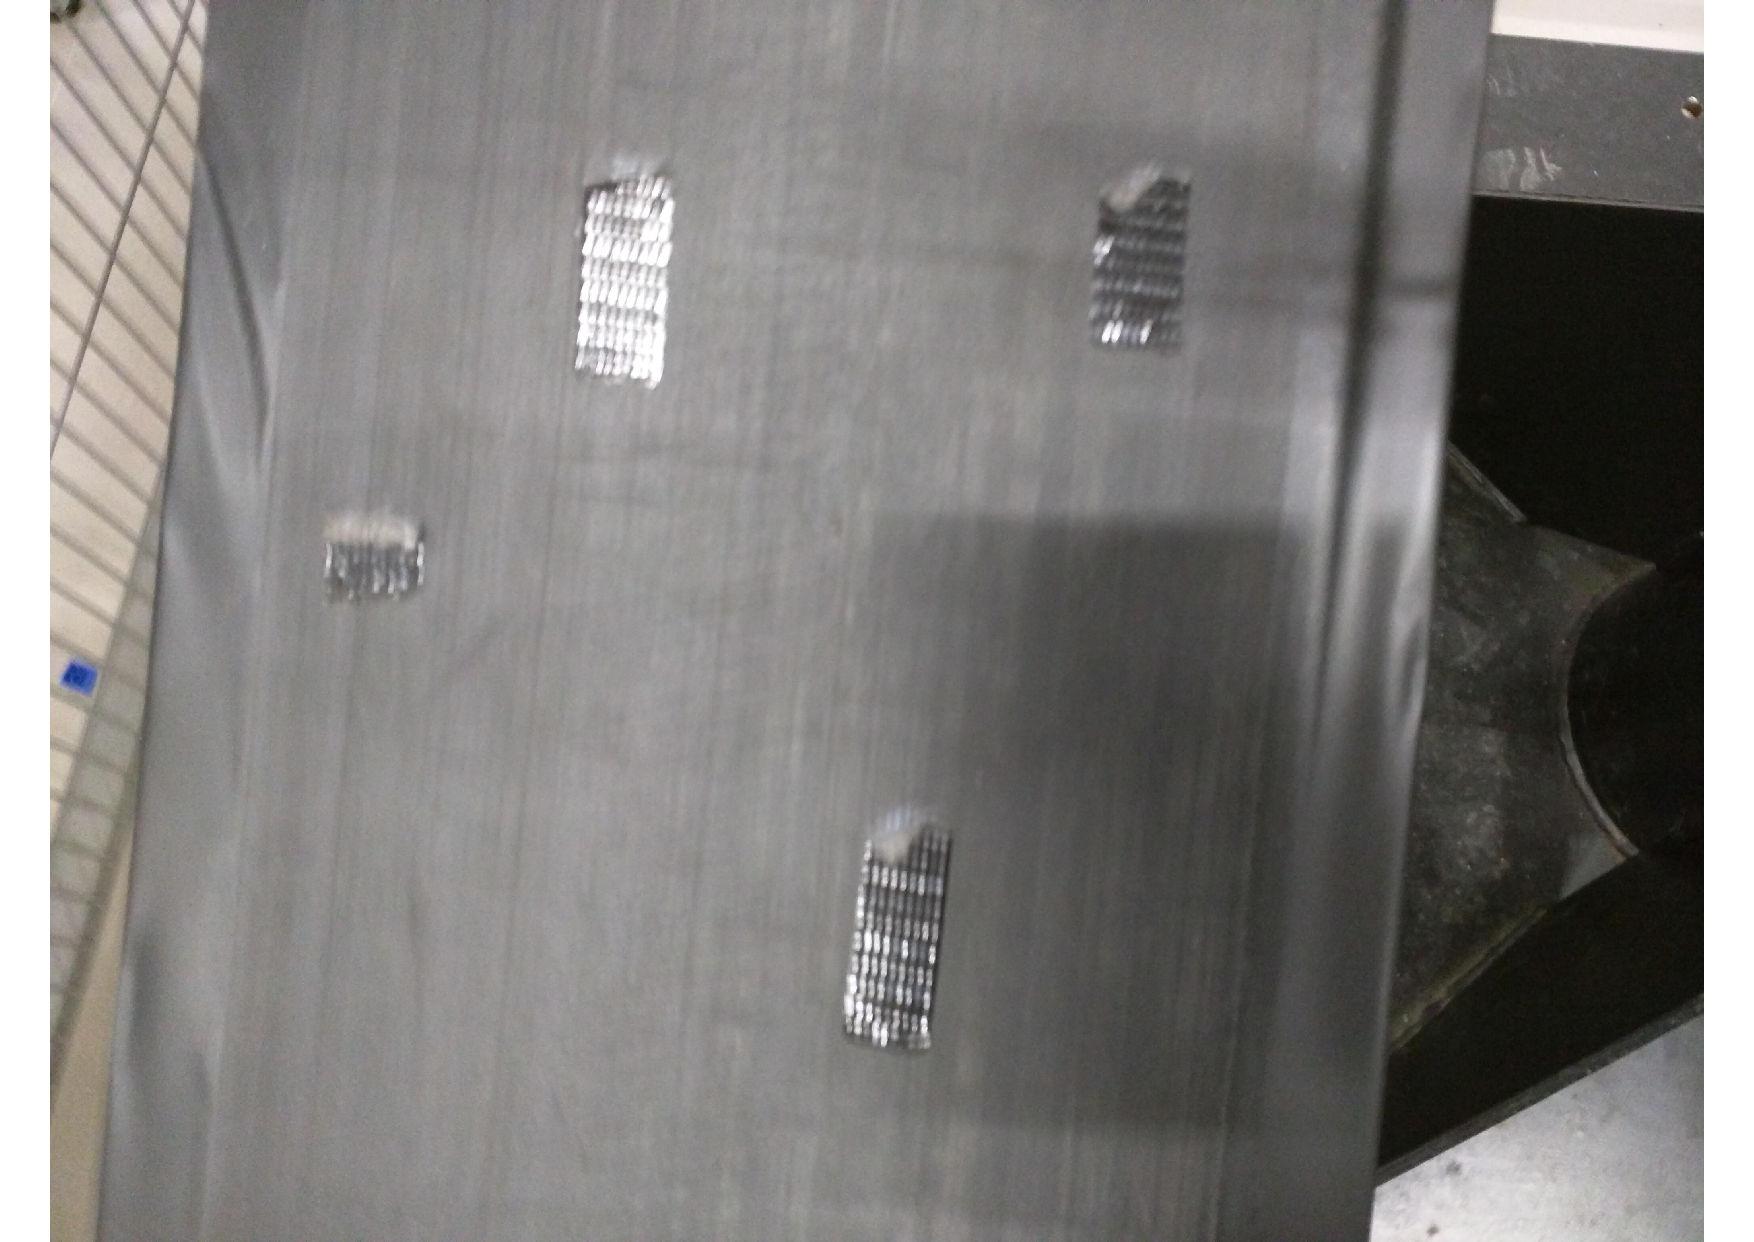
\includegraphics[width=1\textwidth]{duct_tape_rc}
			\caption{Duct tape mounted to conveyor belt}
			\label{fig:duct_tape}
        \end{subfigure}
        \hspace{10pt}
        \begin{subfigure}{0.48\textwidth}
			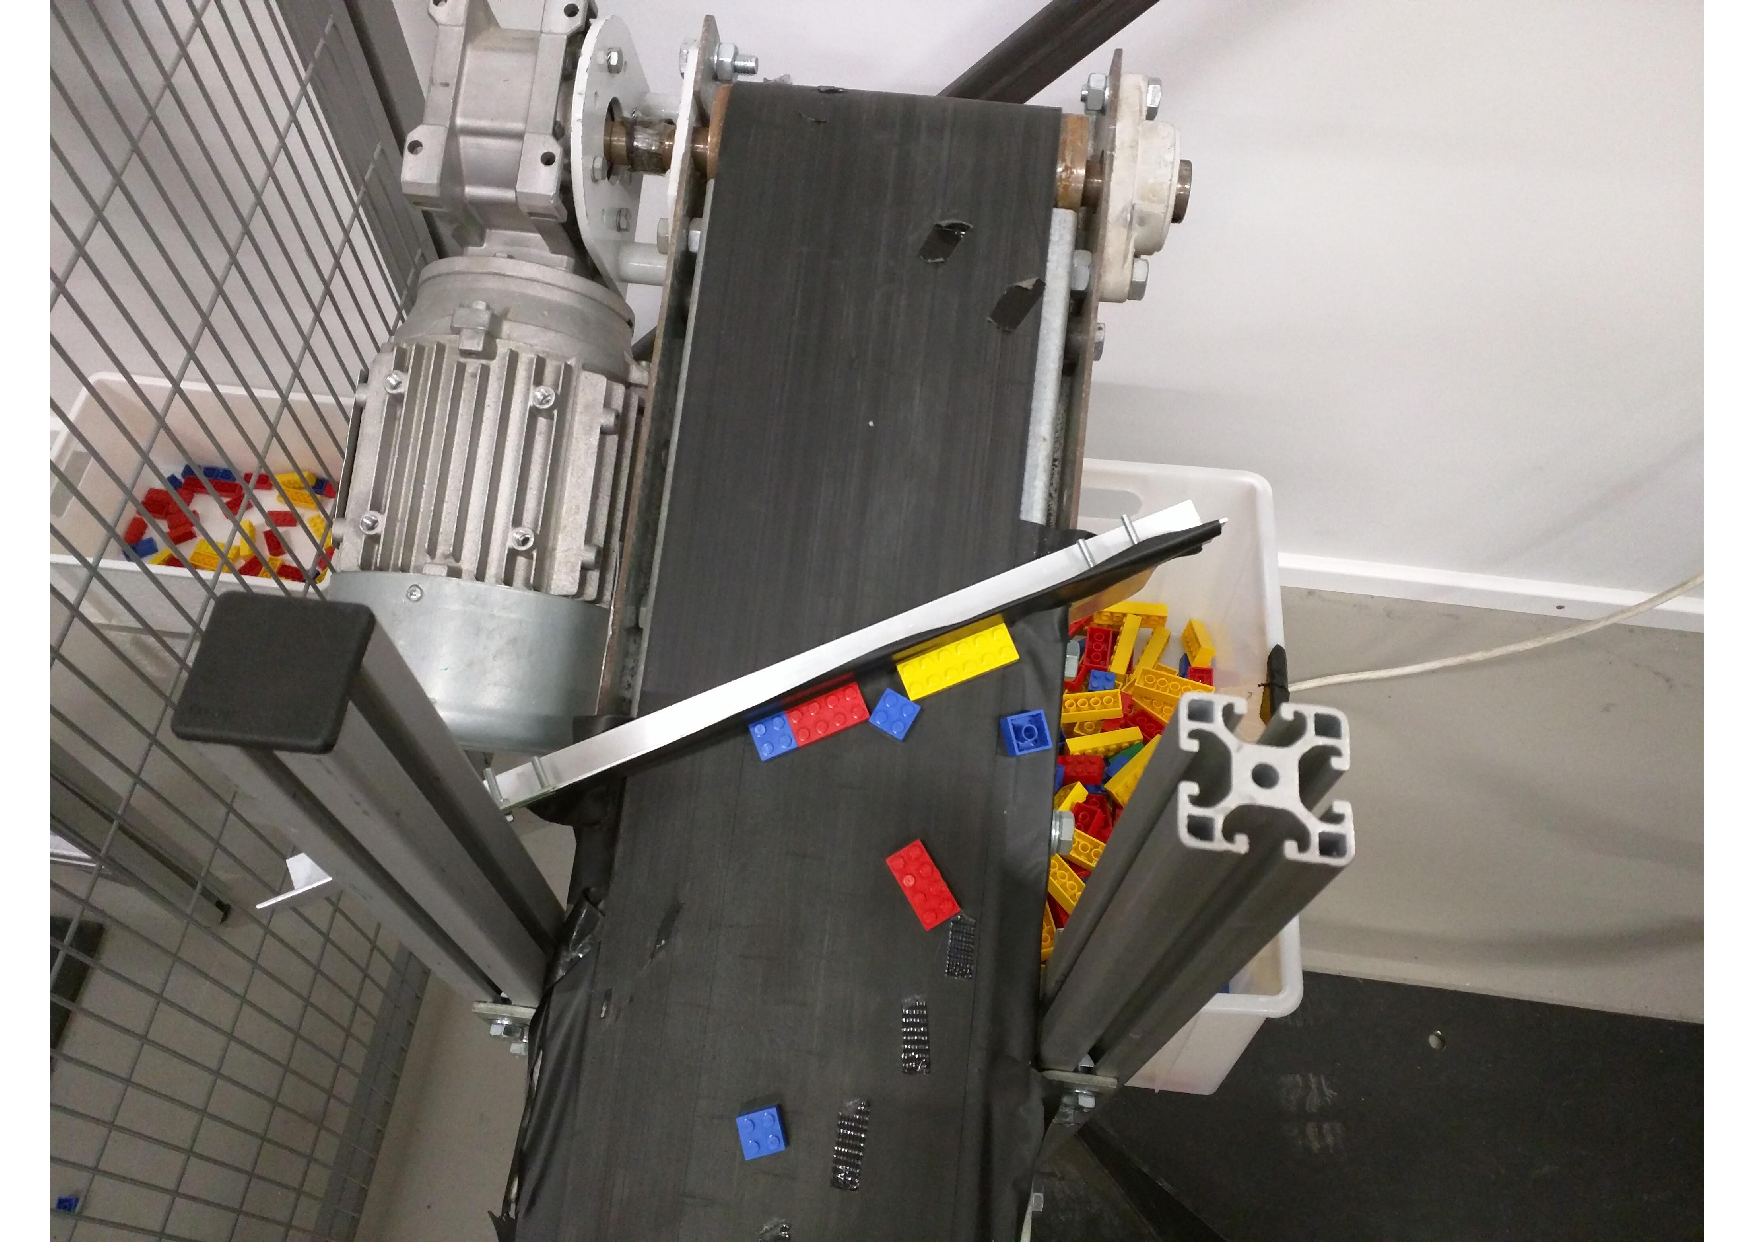
\includegraphics[width=1\textwidth]{slider_to_box}
			\caption{Slider to ensure spare bricks to fall into the box}
			\label{fig:slider}
    \end{subfigure}
    \caption{Example of conveyor modifications}
    \end{figure}

Finally, to avoid unwanted bricks on the floor, a passive slider was mounted near end of the conveyor belt. This allows the bricks to fall into a well placed box and collected at a later time. See figure \ref{fig:slider} 

%!TEX root = ../../../main.tex
%%---------------------------------------------------------------------------
\section{Camera mounting and calibration}
\label{sec:rc_camera}
%%---------------------------------------------------------------------------
The provided camera is a \textit{Logitech webcam C930e}. The camera was mounted on the robot end effector. This was done from the hypothesis that a eye-in-hand camera/robot relationship was easier to calibrate compared to a hand-to-eye system and since there is no concerns with colliding with the camera the view can be closer to the grasping area.

Camera parameters was controlled using the video4Linux api and driver. A resolution of 1280x720 with a 30 FPS was chosen. The resolution was kept high in order to have a rich details in the image and therefore making detecting bricks more stable with a cost of increased computation time due to large image sizes. 
The auto focus of the camera was disabled and the focus was tuned manually since the camera will be fixed in place relative to the bricks.
Brightness, contrast and exposure was also manually tuned in order to capture images with minimum variance. This makes it easier to apply vision algorithms.

Camera calibration was done using the camera\_calibration ROS package. Using this tool the intrinsic parameters of the camera was calculated from images of a 9x7 chequerboard held in front of the camera in 73 different positions. Rectification of the image was then performed using the image\_proc ROS package.

%!TEX root = ../../../main.tex
%%---------------------------------------------------------------------------
\section{Work-cell modelling and calibration}
\label{sec:workcell}
%%---------------------------------------------------------------------------
..

%!TEX root = ../../../main.tex
%%---------------------------------------------------------------------------
\section{Flow control overview}
\label{sec:rc_flow_control}
%%---------------------------------------------------------------------------
	\begin{figure}[H]
		\centering
	    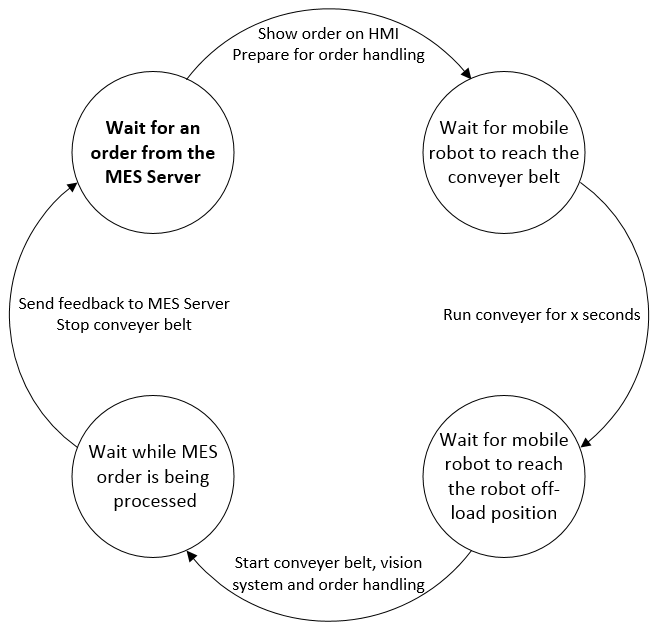
\includegraphics[width=0.75\textwidth]{rc_main_state_diagram}
	    \caption{State diagram of the robot cell}
		\label{fig:rc_main_state}
	\end{figure}
	
	\begin{figure}[H]
		\centering
	    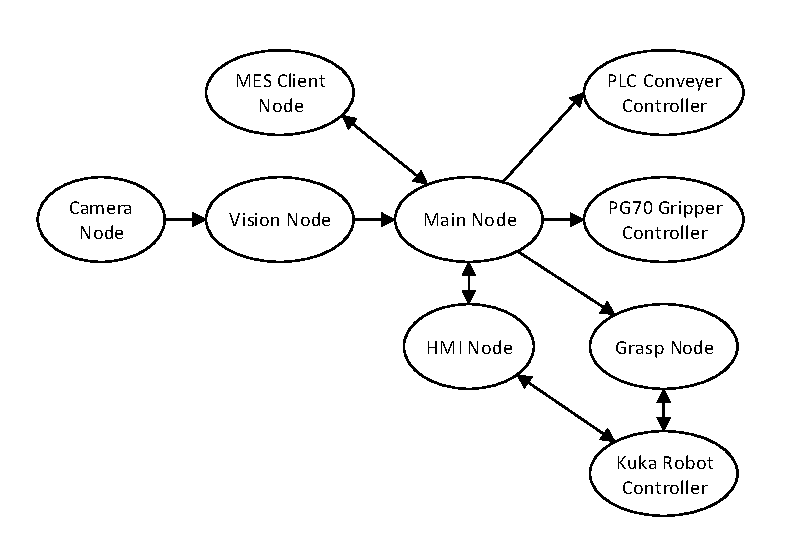
\includegraphics[width=0.8\textwidth]{rc_nodes}
	    \caption{ROS Node structure}
		\label{fig:rc_nodes}
	\end{figure}
	
%!TEX root = ../../../main.tex
%%---------------------------------------------------------------------------
\section{Kuka Robot Controller}
\label{sec:rc_kuka}
%%---------------------------------------------------------------------------
A Kuka ROS node is provided for controlling the robot arm in the robot cell. This makes it possible to communicate and exchange information such as if it is currently moving and what the configuration is. The robot can be moved in configuration space with a given speed and acceleration. \\

ROS services is provided for the above functions and acts as the interface between the Kuka actions and the main application.\\

Some issues were experienced with the Kuka setup when RSI packages was lost due to excess traffic in the switch used to connect the devices. When this occurred the robot controller stopped and the robot could not be moved before a manual reconnection. This situation could be handled by switching the state of the system to \textit{idle}, reconnecting the robot and switching back to \textit{auto}-mode. The system would then continue from the stopping point.

%!TEX root = ../../../main.tex
%%---------------------------------------------------------------------------
\section{Conveyor Belt Controller} 
\label{sec:conveyor_belt_sec}
%%---------------------------------------------------------------------------
The conveyor belt is driven by an AC motor and requires a frequency generator in order to move. The provided frequency generator can either be manually controlled or by a $24V$ digital interface. The interface between the controlling computer and the frequency generator is a PLC. A PLC is an industrial \textit{computer} with $24V$ IO interface and is logic driven. This can be programmed in different ways such as Ladder Diagrams, Structured Text and Function Block Diagrams.\\ 

The PLC in this project is programmed in Structured Text and is simply set up to respond to some serial commands. This makes it possible to start, stop and change the direction of the conveyor belt from an external serial connection.
%!TEX root = ../../../main.tex
%%---------------------------------------------------------------------------
\section{Safety} 
\label{sec:rc_safety}
%%---------------------------------------------------------------------------
The safety in the robot cell consists of a laser beam from Sick mounted in the entrance of the cell. The safety signal is directly connected the Kuka Controller unit and the robot is thus reacting immediately without requiring user interacting. This leaves the conveyor belt, gripper and the Lego sorting system aside. \\

The safety signal can be fetched through the Kuka RSI interface which is provided in ROS format. This allows the system to detect when the safety signal is changing and react upon it. This reaction consists of stopping all actions hereby all physical movements and switching state from \textit{running} to \textit{idle}. The order won't be cleared as such, making it possible to continue when the cell is safe again. \\



%!TEX root = ../../../main.tex
%%---------------------------------------------------------------------------
\section{Vision}
\label{sec:rc_hmi_sec}
%%---------------------------------------------------------------------------
The vision node has the role of detecting Lego bricks on the conveyor belt using the camera. The detection of brick includes the color, size, position and orientation. This is information that is needed in order to determine whether the brick is needed or not and how to grasp it. 

The vision Lego detection algorithm is custom made and consists of several elements from the world of vision. Figure \ref{fig:rc_vision_steps_thor} shows the steps performed on an image in order to search for bricks. These steps are described next.\\
	
	\begin{figure}[H]
		\centering
	    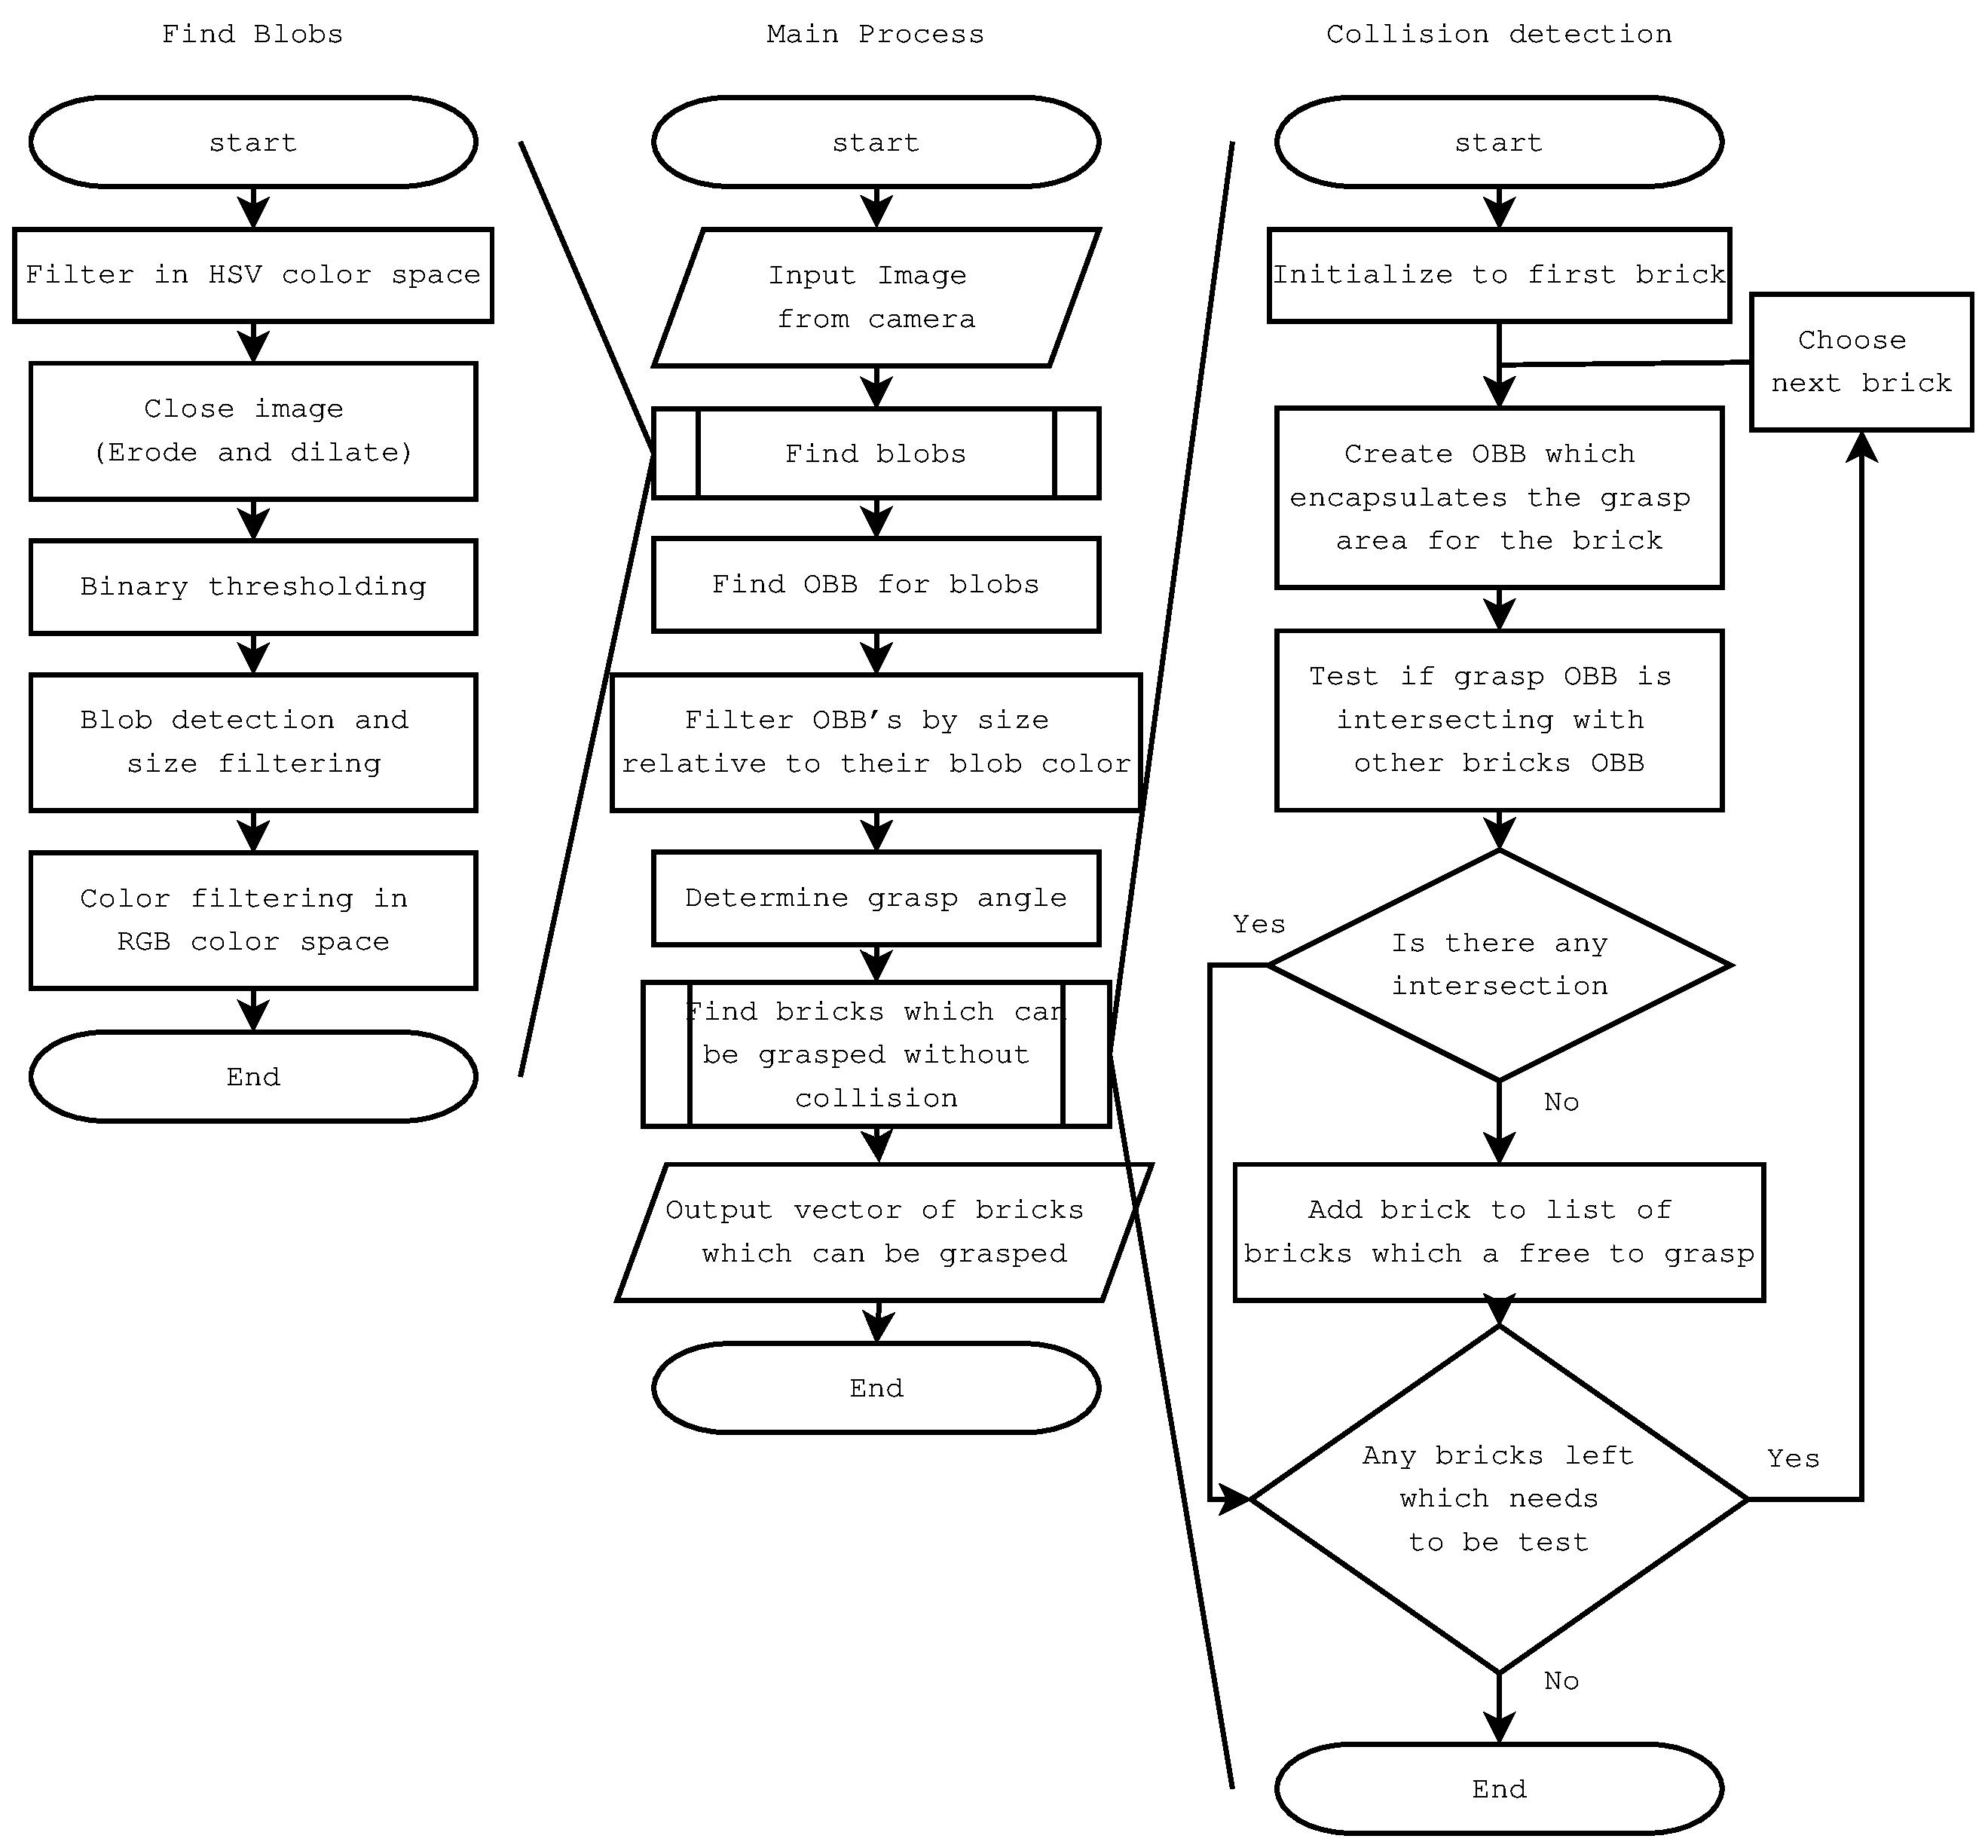
\includegraphics[width=1.0\textwidth]{rc_vision_thor.eps}
	    \caption{Steps to be performed when an image is searched for Lego bricks}
		\label{fig:rc_vision_steps_thor}
	\end{figure}
	
The vision node is able to deliver two services. One that uses a quick method to tell whether or not any bricks can be seen in the image and one that describes the image in full detail with all relevant brick information. This is used in order to save calculation time since there is no need to request the full vision algorithm if there is no bricks.

The quick method consists of only the left \textit{find blobs} part in figure \ref{fig:rc_vision_steps_thor}. This involves filtering in HSV space in order to separate the background elements from the Lego bricks. Then the image is \textit{closed} which consists of the erode and dilate process. A binary threshold is applied in order to get a binary representation of the image which is needed in blob detection. The blob detection algorithm detects the connected pixels in the image and separates them as blobs. The blobs are size filtered in order to get rid of small noisy contours. Lastly the color of the blob is determined by a custom color detection algorithm. The average RGB pixel value of all the pixels belonging the blob is calculated and the amount that the respective colors present in percentage with respect to the sum determine the correct color. Looking at the amount that the colors make up, a conclusion of the color can be made. This is robust with respect to changing light conditions and other changes to the colors. 

The next step looks into fitting oriented-bounding-boxes (OBB) to the blobs, using an OpenCV\cite{opencv} implementation. This results in the size, orientation and center position of the detected element. The size and color combination is used for further brick filtering.

The orientation of the bricks is always with respect to the y-axis of the frame and smallest side of the bricks. This makes it easy for grasp calculation and the smallest side is chosen since some Lego bricks can be too large for grasping on the longest side. 
	
	\begin{figure}[H]
		\centering
	    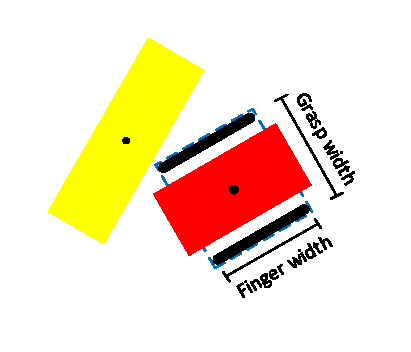
\includegraphics[width=0.5\textwidth]{rc_vision_collision.pdf}
	    \caption{Lego brick collision detection method}
		\label{fig:rc_vision_collision}
	\end{figure}
	
Finally collision avoidance is done by testing if any obstacles is in the grasp path for a brick. The grasp path for a brick is the area the two fingers of the end effector travels when trying to grasp the brick. Figure \ref{fig:rc_vision_collision} shows a example where the two bold black lines illustrates the end effector fingers. The area encapsulated by the stripped blue lines is the grasp path area for the grasp when trying to grasp the red brick illustrated by a red rectangle. A grasp path area is then tested against all other bricks except the brick to be grasped. Separating axis theorem\cite{Gottschalk:1996:OHS:237170.237244} is used to test if the rectangular grasp area is colliding with the rectangular brick areas defined by OBB's.

Since the positions of the bricks are found in the image and thus in pixels, it needs to be translated to the distance metric that the robot and gripper are using, namely meters. The pixel to meter conversion was archived using a simple method in which four corner points were marked on the conveyor and the distance between these was measured. The same distance was measured on the image in pixels. The different measurements was summed and the average scale found. It was assumed that if the set-up was kept static the scale would be valid for a longer period.

Figure \ref{fig:rc_vision_ex1} and \ref{fig:rc_vision_ex2} shows two results of the vision algorithm. The white box defines the area that a brick can be picked within. The contour of a detected brick is drawn with the color detected. The width of the contour if either thick or thin. Thick illustrates that the brick is pick-able thus not in collision and within the workspace. The green color marks a \textit{monster}, a brick or collection of bricks that is not detected as a valid brick. 

  	\begin{figure}[H]
        \centering
        \begin{subfigure}{0.45\textwidth}
            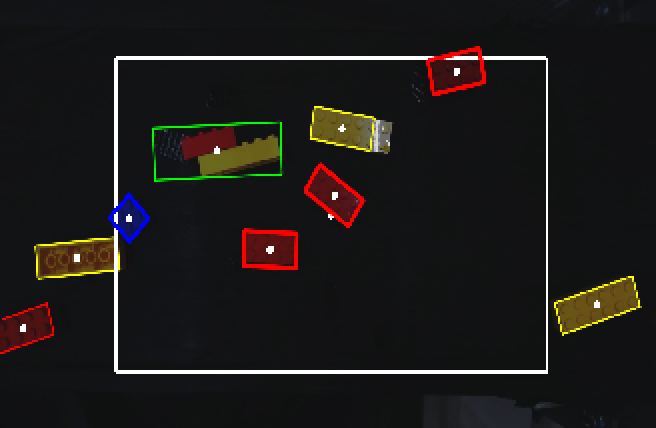
\includegraphics[width=\textwidth]{figs/rc_vision_ex1}
            \caption{}
            \label{fig:rc_vision_ex1}
        \end{subfigure}
        \hspace{10pt}
        \begin{subfigure}{0.45\textwidth}
            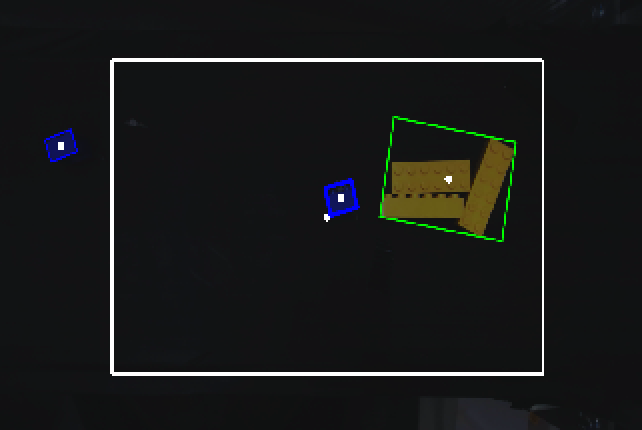
\includegraphics[width=\textwidth]{figs/rc_vision_ex2}
            \caption{Two blue bricks and a \textit{monster}}
            \label{fig:rc_vision_ex2}
    \end{subfigure}
    \caption{Example of vision output}
    \end{figure}
%!TEX root = ../../../main.tex
%%---------------------------------------------------------------------------
\section{Robot motion and grasping}
\label{sec:rc_grasp}
%%---------------------------------------------------------------------------
When a brick is detected and is in agreement with the order it needs to be picked and moved from the conveyor belt to the tipper of the mobile robot. This requires a number of robot and gripper actions. 

Figure \ref{fig:rc_grasp} shows the steps taken when a brick is to be picked. 

	\begin{figure}[H]
		\centering
	    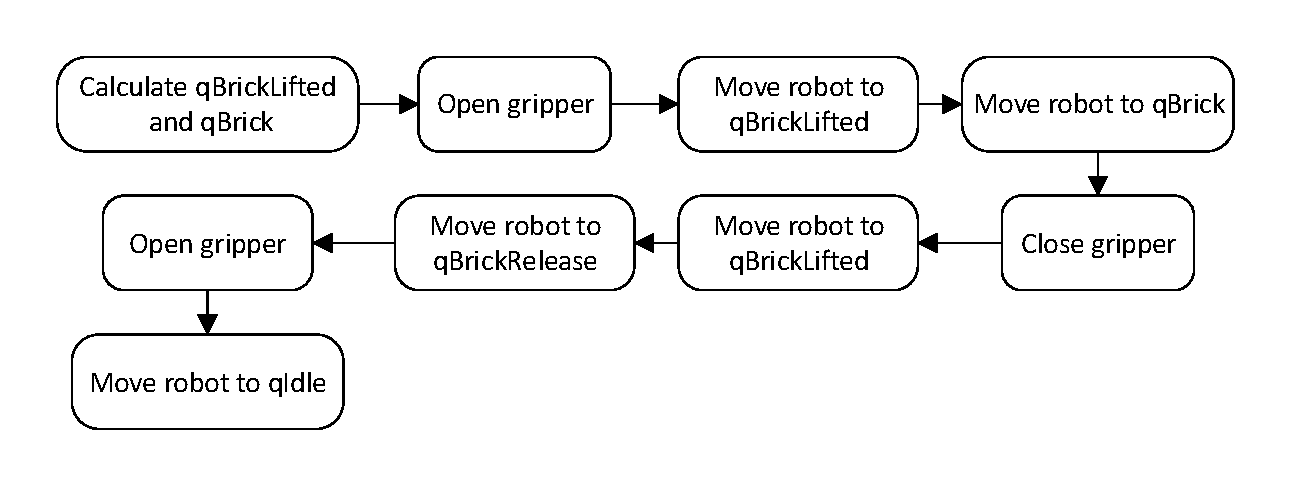
\includegraphics[width=0.95\textwidth]{rc_grasp_steps}
	    \caption{Steps performed when a Lego brick is to be picked}
		\label{fig:rc_grasp}
	\end{figure}
		
The idle position of the robot is with the z-axis of the camera frame aligned with the z-axis of the conveyor frame but with a certain distance displacement, as seen in figure \ref{fig:rc_frames}.

The calculation of \textit{qBrickLifted} and \textit{qBrick} includes inverse kinematics calculations used in order to get the position of the brick in the conveyor frame to a position in the robot frame with respect to the gripper. The configurations respectively represents the one in which the gripper and robot is aligned for grasping, but with a small offset in the z-axis and the configuration without the z-axis offset in which the gripper is in position for closing.  

No path planning is used in the process since the work-cell is static. The area in which bricks can be picked from is limited thus eliminating wrongly detected bricks resulting in collision. 


%!TEX root = ../../../main.tex
%%---------------------------------------------------------------------------
\section{Main Control}
\label{sec:rc_main}
%%---------------------------------------------------------------------------
The main component in the system is the one responsible for running the brick sorting application. The MES order is delivered to the main and it is responsible of performing the corresponding actions and starting the required services.

The brick sorting loop is only running when an order is present, the auto-mode is set, the security is okay and the robot is at the idle position. If that is the case the conveyor belt is started and the vision rough brick detector activated. When a brick is detected, the full algorithm is performed in order to match a brick with one requested in the order. The conveyor belt is only stopped if this is the case. This makes the brick sorting quite fast since a stop in the flow only occurs when a brick is to be picked. 

A security stop will at any time result in a change to idle mode and a stop of all actions. 
%!TEX root = ../../../main.tex
%%---------------------------------------------------------------------------
\section{Human Machine Interface}
\label{sec:rc_hmi}
%%---------------------------------------------------------------------------
A separate Human Machine Interface (HMI) is developed for controlling the robot cell. This allows the user to control relevant parameters from an intuitive GUI. 

The HMI is implemented as a plugin to RobWorkStudio. This allows the HMI to act alongside the visual representation of the work-cell allowing a real-time simulation of the actions.

Figure \ref{fig:rc_hmi} shows the HMI plugin. All system elements are using the log for error and information messages. The user is able to manually control the robot, conveyor and gripper. Some camera settings can be directly controlled from the HMI and the video feed shows a direct view of either the raw or vision applied image. 

	\begin{figure}[H]
		\centering
	    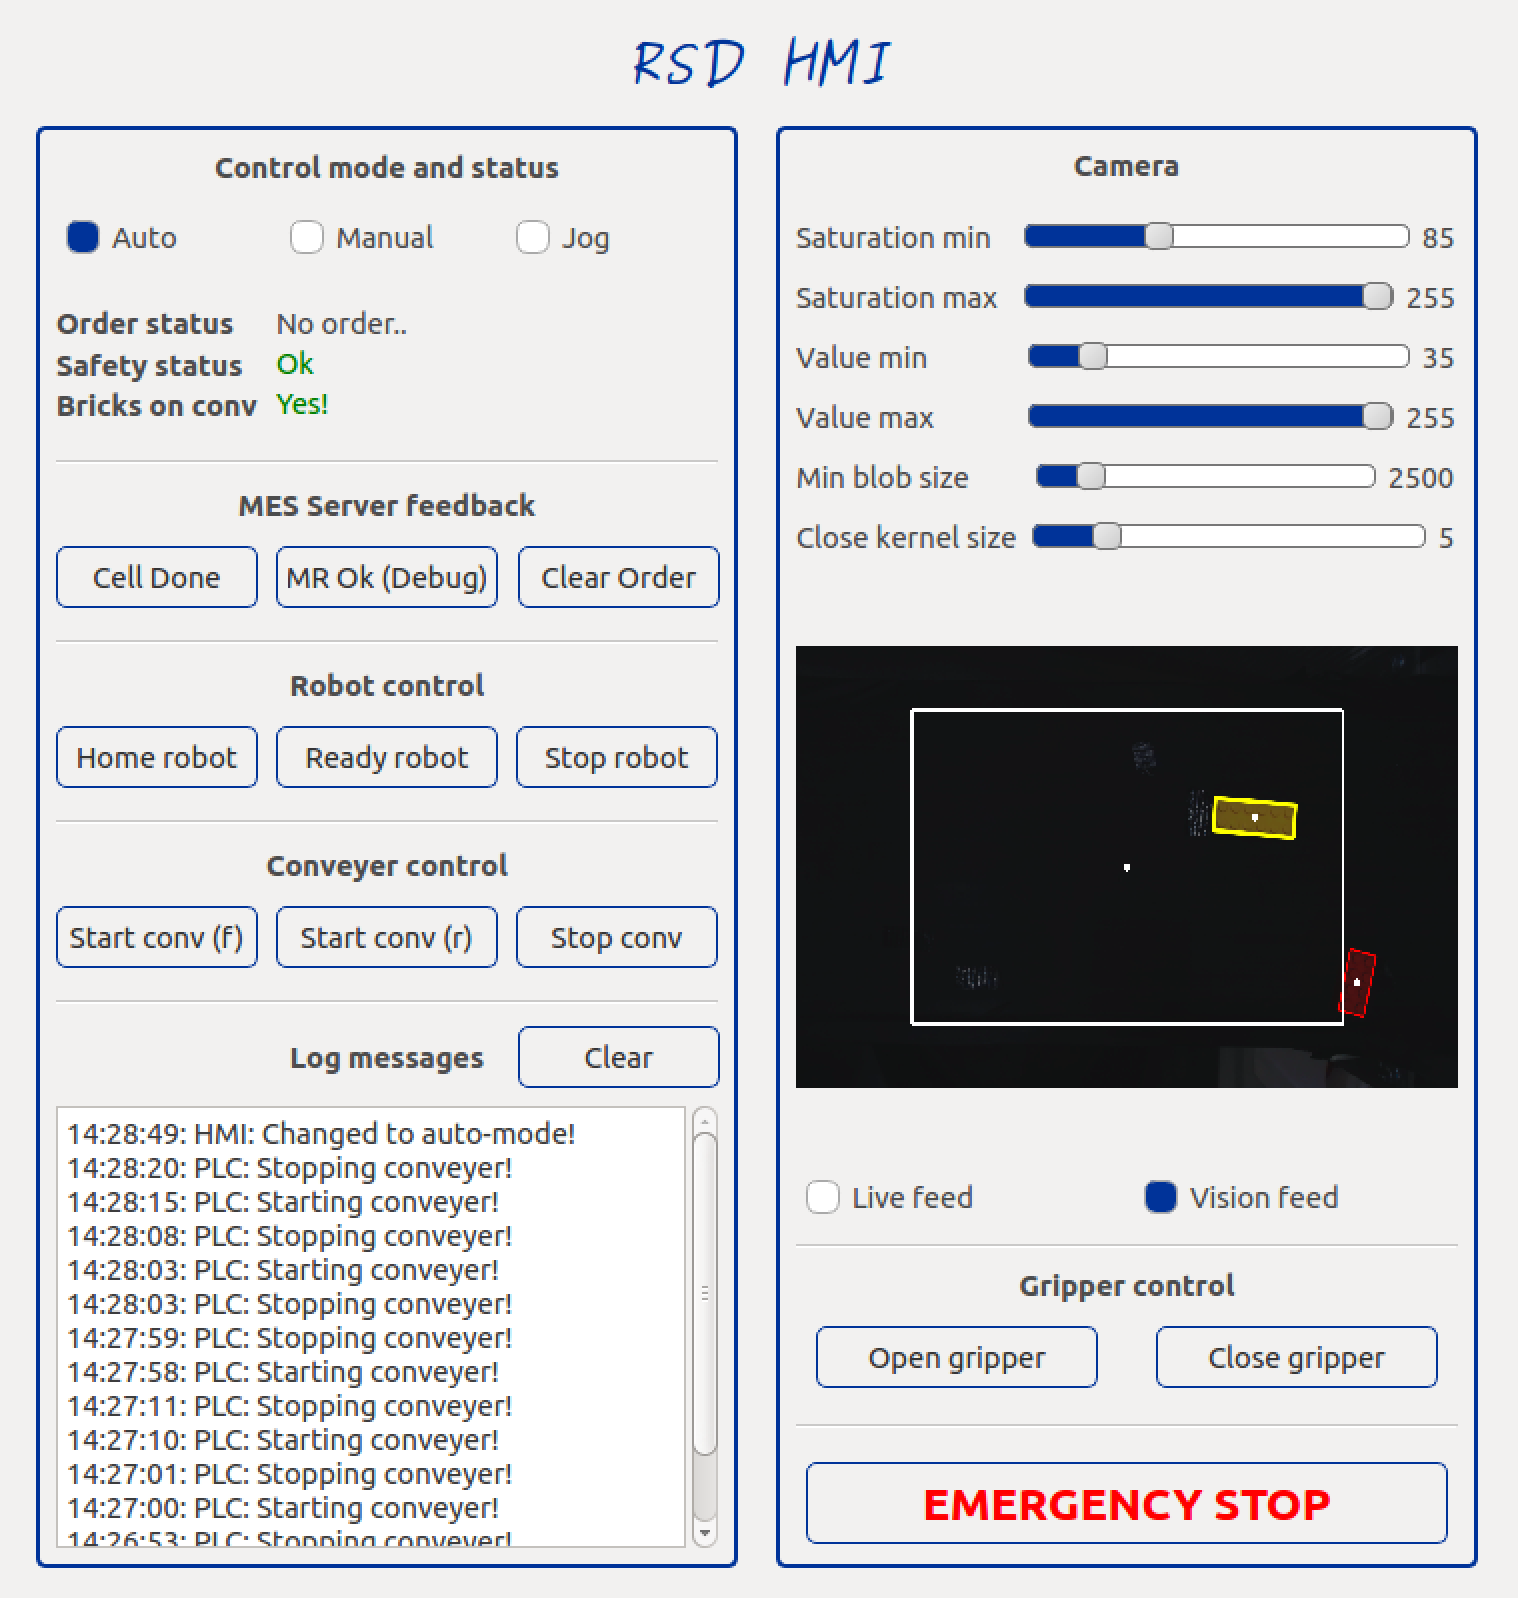
\includegraphics[width=0.9\textwidth]{rc_hmi}
	    \caption{HMI}
		\label{fig:rc_hmi}
	\end{figure}


%%% Local Variables:
%%% mode: latex
%%% TeX-master: "main"
%%% End:
    %!TEX root = ../../main.tex
%----------------------------------------------------------------------------
\chapter{Financial Aspects}\label{chap:financial_aspects_chapter}
%----------------------------------------------------------------------------
The up and coming start-up "Super Smart SDU Robotics Graduates A/S" is planning to expand into a new business area. For this, the idea is to set up a a fully automated LEGO Bricks sorting and packaging line. People will be able to send in their old LEGO bricks and get paid by weight. The income comes from customers ordering very specific combinations of LEGO bricks at a far lower price point than ordering them directly at LEGO or at a toy store. 

	\begin{figure}[H]
        \centering
        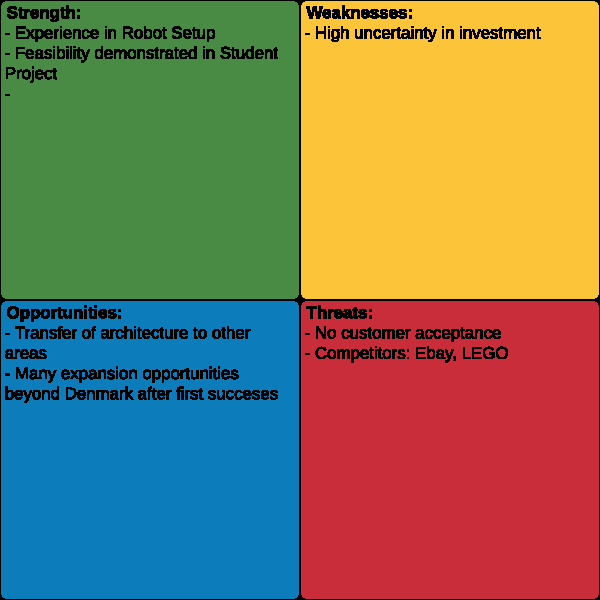
\includegraphics[width=0.6\textwidth]{swot}
        \caption{SWOT-Analysis}
        \label{fig:swot}
    \end{figure}
    
The SWOT-Analysis was done within the management and an external consultant as seen in figure \ref{fig:swot}
\begin{table}[]
\centering
\begin{tabular}{llll}
\textbf{Name}          & \textbf{Type} & \textbf{Cash Flow} & \textbf{Anual increase} \\
Kuka Robot             & one-time      & -250.000           &                         \\
Frobit Robot           & one-time      & -100.000           &                         \\
Set-up labor cost      & one-time      & -300.000           &                         \\
Maintenance - Hardware & anual         & -10.000            & 4\%                     \\
Maintenance - Labor    & anual         & -78.000            & 5\%                     \\
Income                 & anual         & 250.000            & 10\%                   
\end{tabular}
\caption{Market Research}
\label{tab:market_research}
\end{table}
A careful organized market research has been done to analyse the feasibility of said proposal. These results of the market research, table \ref{tab:market_research}, shows both the potential annual income as well as estimated investment cost.
The labour cost are based on an engineering salary of DKK $1.500$ per hour. For the set-up, $200$ engineer-hours are budgeted and for maintenance one hour per week. Salary is set to increase by $5\%$ and the maintenance annually by $4\%$. These values are chosen very conservative (above the raw material price index for maintenance material and above the average salary increase over the past five years) to allow for fluctuation and uncertainties. \\ 
The income growth over the first five years is set to constant $10\%$ even though a steeper increase is expected after the first market penetration.\\
    \begin{figure}[h]
        \centering
        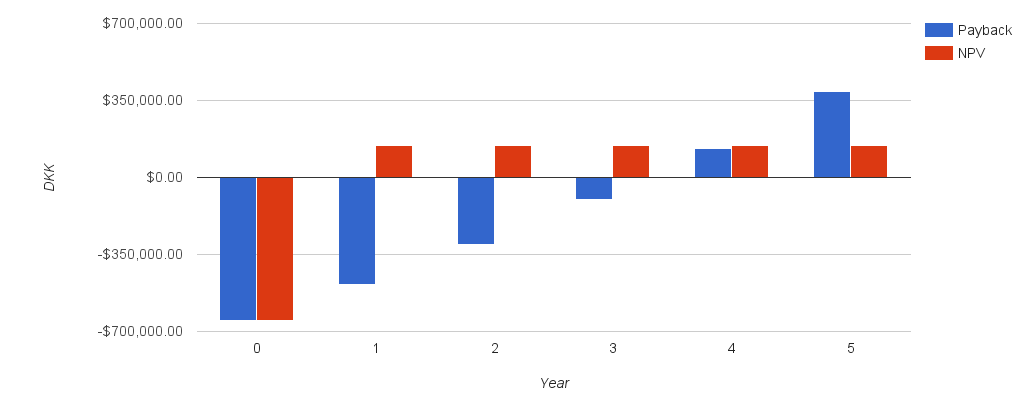
\includegraphics[width=1.0\textwidth]{figs/pb_npv}
        \caption{Payback Method and Net Present Value}
        \label{fig:payback_npv}
    \end{figure}

Given these assumptions the pay-back method \ref{fig:payback_npv} (blue), the internal rate of return method (IRR) and the net-present value (NPV) \ref{fig:payback_npv} (red) are calculated to determine the feasibility of this investment.
The pay-back method shows a profit of DKK $390.000$ after five years. The investment was judged as having a medium risk, but for calculating the NPV the required rate of return of investment has been set to $12\%$ to be conservative. With this the NPV of this investment after considering five years with the given assumptions would be DKK $80.000$ and thus the investment is seen as favourable. The IRR is $16.47\%$ , this far exceeds simply investing in bonds, or paying back current bank loans, of which the highest is DKK $2.000.000$ at $7\%$.
All methods suggest this investment is profitable and the financial department gives the project the go-ahead.

%%% Local Variables:
%%% mode: latex
%%% TeX-master: "main"
%%% End:
    %!TEX root = ../../main.tex
%----------------------------------------------------------------------------
\chapter{System Test}\label{chap:system_test_chapter}
%----------------------------------------------------------------------------

% Please keep sections separated in their designated folders and only reference them here using the input tag

In order to prove the capabilities of out design and to bring all the so far undetected bugs and errors to light, we were asked to perform a 24-hour integration test. During this 24 hours, all components of the system had to be used throughout multiple iteration of the brick selection and delivery procedure. 

Since the timespan of the test was such that it encapsulated a whole day, the systems had to cope with changing light conditions, continuous interference by human operators and spectators moving around them, the degradation of markers essential for navigation while being forced to interact with other system components, the mobile platforms of the other groups. In the following sections we present a detailed description of the tests we performed, the results we got and their evaluation.


\section{Test description}

In the beginning of the test, all mobile platforms were situated at the charging stations, fully charged. One iteration consisted ot the following milestones:

\begin{enumerate}
	\item Leaving the charging station in a fully charged state and taking up position under the LEGO dispenser machine
	\item Waiting for the bricks to be loaded on the tipper (since the dispenser was not operational, we just simulated the process)
	\item Delivering the LEGO to the robot cell
	\item Unloading the bricks to the conveyor belt
	\item Moving the bricks into position for selection through robotic vision
	\item Picking the LEGO bricks specified by the order (this is equivalent to loading them on the mobile platform)
	\item Trafficking the LEGO back to the box, and docking at the charger
\end{enumerate}

All components of the system were continuously broadcasting location and status information, which was displayed on the HMI, while the map used for SLAM navigation and the console-printed ROS information were also monitored. We compared all these with the actual position and behavior of the system components, logged their performance, and intervened when errors occurred. 

\section{Log}

We logged the date and time, the person  responsible for creating the entry, the type of the entry and a short note describing the reason for making it.

We have distinguished between the following types:

\begin{itemize}
	\item Order Start
	\item Order Finish
	\item Error
	\item Manual Shutdown
	\item System Event
	\item Other
\end{itemize}


\section{Test results}

Even though in the initial phase camera connection issues caused delays in the testing process, all in all 49 iterations were performed, out of which 36 were finished successfully resulting in a success ratio of 73.47\% (see Figure \ref{fig:order_statistics} ).

\begin{figure}[H]
    \centering
    \begin{subfigure}[b]{0.48\textwidth}
        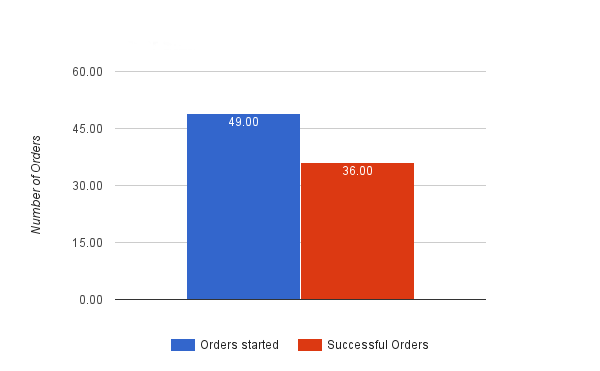
\includegraphics[width=\textwidth]{order_statistics}
        \caption{Order statistics}
        \label{fig:order_statistics}
    \end{subfigure}
    ~
    \begin{subfigure}[b]{0.48\textwidth}
        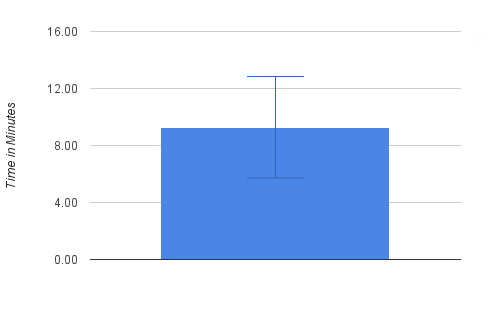
\includegraphics[width=\textwidth]{execution_time}
        \caption{Execution time}
        \label{fig:execution_time}
	\end{subfigure}
\caption{Test statistics}
\end{figure}

We managed to improve the speed of the system throughout the testing and on average we achieved an execution time of  9.28 minutes with a standard deviation of 3.35 (see Figure \ref{fig:execution_time}).

The two main sources of errors we have observed were originated in inter-component communication and the localization of the mobile platform. Since both are effected greatly by external factors such as congestion and uncontrollable changes in the environment caused by human and mobile robot movement, they cannot be mitigated without introducing fundamental changes to the design. 

Nevertheless, the fact, that after the initial difficulties no mayor errors occurred shows, that the corrected system is mostly bug free and a capable solution for the task presented.





%%% Local Variables:
%%% mode: latex
%%% TeX-master: "main"
%%% End:
    %!TEX root = ../../main.tex
\chapter{Discussion}
\label{chap:discussion}
In this chapter the discussion about the final status of the project, as well as future work or improvements, is presented.
Following the structure of the report this is divided in two parts: (1) the mobile robot and (2) the robot work-cell.

	\section{Mobile robot} % (fold)
	\label{sub:mobile_robot}
	Based on the results presented in the section \ref{chap:system_test_chapter}, some hardware proposals are suggested:
	\begin{itemize}
		\item Have better space awareness, perhaps, given two LIDARS.
		\item Improve runtime. This can be achieved either with better batteries or reducing the power consumption.
		\item Improve reliability of the tipper. Perhaps improving the materials and the building quality of the assembly.
		\item Use global shutter cameras so the motion blur can be reduced. This will allow to detect QR when moving fast avoiding have to stop to read the data.
		\item Improve the mechanical implementation of the robot to increase robustness and reliability of the robot.
		\item Make a more modular robotic platform in order to let the user to change the shape of the robot to adjust it to the personal purposes.
		\item Having the camera localization inside the box will help to have a more robust position of the robot.
	\end{itemize}
	And as an improvement in the software side:
	\begin{itemize}
		\item Improve free navigation. An option could be have several local path planner for the different purposes in the free navigation.
		\item The relative navigation can be improved using a PID implementation.
		\item The HMI can be improved in the UI side as well as the functionality. A web service for controlling not only the mobile robot, but the robot work-cell and the MES Server can be done.
		\item The general speed of the robot can be increased in order to increase the productivity.
	\end{itemize}
	% section mobile_robot (end)

	\section{Robot workcell} % (fold)
	\label{sub:robot_workcell}
	
	The role of the robot cell was to simply detect and select the bricks that matched the order sent by the MES Server. This was executed by the vision detection task and the grasping task using the gripper and robot. 

The vision algorithm being able of detecting and identifying bricks while the conveyor belt was running, performed good. A precise calibration of the scene, camera and gripper was done resulting in no erroneous grasps. The vision was independent of daylight fluctuation and no brick was marked collision-free while not being so.

There is however room for improvements. The current implementation of the system allows only grasps on the center of the thin side on the bricks. This results in a large number of bricks being ignored due to a grasp attempt will lead to collision. 

In order to increase the speed of the brick sorting the following can be considered. 
The speed of the gripper closing and opening was quite slow. Increasing this would led to faster brick selection. 
A suction based gripper would allow bricks to be picked even if no clear area is available around the brick. This requires the vision to be able to distinguish between bricks even if a bunch of same-coloured bricks are presented. 

A more low-level solution could consist of a better hardware set-up that results in more separated bricks thus allowing more bricks to be picked. 

Finally in order to increase multitasking, an eye-to-hand mounting of the camera could have been chosen. This would allow the robot to grasp and move bricks while the vision could analyse the next move. 

% section robot_workcell (end)j
    %!TEX root = ../../main.tex
%----------------------------------------------------------------------------
\chapter{Conclusion}\label{chap:conclusion}
%----------------------------------------------------------------------------
1. Jorge fra Pjort 
Jorge fra Pjort, 
han flyver længere og længere bort 
på sin fantastiske flyvende færd. 
Hodja ka’ ik’ la’ vær’ 
før han har set, hvordan hele verden er. 



2. Faza fra Pjort, 
Faza fra Pjort, 
gav ham det tæppe, der førte ham bort 
henover landet fra syd og til nord. 
Hodja det’ no’et du tror, 
troen kan hæve dig højt fra denne jord. 



Østen for solen og vesten for månen, 
syv vilde vinde skal bære dig 
østen for solen og vesten for månen. 

3. Hodja pas på, 
Hodja pas på, 
det bedste du har, gør de alt for at få. 
Ho’derne ruller- din sultan er sur, 
rotterne står på lur, 
stjæler dit tæppe og låser dig i bur. 


4. De sir halvfjerds 
mærk’lige vers, 
prøver det både på kryds og på tværs. 
Det flyvende tæppe, det blev hvor det lå 
- det ku de ik’ forstå - 
Hodja er sikkert den eneste, der må. 


5. Hodja blev fri, 

Hodja slap fri, 

kaldte på tæppet og fløj li’ forbi. 

Sultanen faldt på sit haleparti 

det gjorde ondt fordi: 

ingen skal stjæle fra børnenes fantasi. 



Østen for solen…



6. Som 1. vers 


The robot cell developed is able to; receive unsorted bricks from the mobile platform, pick the correct bricks according to order specification from MES server and placing the order back on the mobile robot. All this functionality can operate automatically or supervised by an user through the developed HMI. The 24 hour integration test showed a fairly stable Robot cell system with mostly minor errors which could be resolved and recovered from manually.

%test showed 9 errors with the robot cell out of 49 runs. 3 of the errors were resolved during the test, 3 errors was from external issues which the group have no control of. The last three 



%%% Local Variables:
%%% mode: latex
%%% TeX-master: "main"
%%% End:

    \titlespacing*{\chapter}{0pt}{6pt}{5pt} % Sets the space before and after the title declaration
    % references section
    \bibliographystyle{sty/IEEEtranBST/IEEEtran}
    \bibliography{bib/IEEEabrv,bib/references,bib/platforms}\thispagestyle{empty}

    \appendix
%\begin{appendices}
	%----------------------------------------------------------------------------
\chapter{}
%----------------------------------------------------------------------------

\section{Buttons board's LED meaning} % (fold)
\label{sec:buttons_board_s_led_meaning}

\begin{itemize}
	\item \textbf{White, not blinking}: The robot is in \emph{idle} mode.
	\item \textbf{Green, blinking}: The robot is in \emph{auto} mode.
	\item \textbf{Purple, blinking}: The robot is in \emph{manual} mode.
	\item \textbf{Yellow}: The robot is in \emph{proximity alert}.
	\item \textbf{Red}: The robot is in \emph{collision}.
\end{itemize}

% section buttons_board_s_led_meaning (end)
	%%----------------------------------------------------------------------------
\chapter{}
%----------------------------------------------------------------------------

%\end{appendices}


    %\clearpage
    %\listoftodos

\end{document}